\documentclass{article}
\usepackage{microtype,graphicx,booktabs,multirow}
\usepackage{hyperref}
\usepackage{xurl}
\newcommand{\theHalgorithm}{\arabic{algorithm}}
\usepackage{icml2026}
\usepackage{amsmath,amssymb,mathtools,amsthm}
\usepackage{algorithm,algorithmic}
\usepackage[capitalize,noabbrev]{cleveref}
\hypersetup{pdftitle={Midpoint Generative Models for General Geometries},pdfauthor={},pdfsubject={Research draft; experimental snapshot 26 October 2026}}
\newtheorem{theorem}{Theorem}[section]
\newtheorem{proposition}[theorem]{Proposition}
\newtheorem{corollary}[theorem]{Corollary}
\newtheorem{lemma}[theorem]{Lemma}
\theoremstyle{definition}
\newtheorem{assumption}[theorem]{Assumption}
\newtheorem{definition}[theorem]{Definition}
\theoremstyle{remark}
\newtheorem{remark}[theorem]{Remark}
\crefname{assumption}{Assumption}{Assumptions}
\Crefname{assumption}{Assumption}{Assumptions}
\newcommand{\M}{\mathcal M}
\newcommand{\R}{\mathbb R}
\newcommand{\E}{\mathbb E}
\newcommand{\D}{\mathcal D}
\newcommand{\Lcal}{\mathcal L}
\newcommand{\Exp}{\operatorname{Exp}}
\newcommand{\Log}{\operatorname{Log}}
\newcommand{\Law}{\operatorname{Law}}
\newcommand{\grad}{\operatorname{grad}}
\newcommand{\Tr}{\operatorname{tr}}
\newcommand{\RMGM}{\textsc{R-MGM}}
\newcommand{\norm}[2]{\lVert #2\rVert_{#1}}
\newcommand{\dd}{\,\mathrm d}
\icmltitlerunning{Midpoint Generative Models for General Geometries}
\begin{document}
\twocolumn[
\icmltitle{Midpoint Generative Models for General Geometries}
\begin{icmlauthorlist}
\icmlauthor{Anonymous Authors}{anon}
\end{icmlauthorlist}
\icmlaffiliation{anon}{Anonymous Institution}
\icmlcorrespondingauthor{Anonymous Author}{anon.email@domain.com}
\icmlkeywords{Generative modeling, Riemannian geometry, midpoint divergence, one-step generation}
\vskip 0.3in
]
\printAffiliationsAndNotice{}
\begin{abstract}
We introduce Riemannian Midpoint Generative Models, which train a manifold-valued one-step generator using a tangent regression critic and randomly flipped geometric interpolations. For reversible finite-energy paths, we prove that the intrinsic discrepancy is symmetric, vanishes exactly when its endpoint distributions agree, and upper-bounds squared Wasserstein-1 distance. Its variational form gives alternating training, with simulation-free interpolation where closed-form paths are available and no learned flow integration at inference. A nine-task controlled study exposes finite-critic optimization failures, while a partial comparison with recent one-step methods does not establish practical superiority. In a completed two-object SE(3) pilot, midpoint generation improves pose MMD over an adapted one-step MeanFlow but remains less accurate than multi-step RFM and has substantial gripper collisions. These results distinguish population discrepancy guarantees, successful finite-network learning, and downstream physical feasibility.
\end{abstract}
\section{Introduction}
Generative models are increasingly asked to produce objects whose admissible values form a curved or constrained space. Geographic locations lie on a sphere; torsion angles are periodic; covariance matrices must remain positive definite. An ambient Euclidean model can place probability outside the domain, and a final projection can distort the learned distribution. A useful construction should therefore address two distinct questions: how the output is constrained, and how the training objective uses the geometry of the data.

Riemannian Flow Matching (RFM) learns a time-dependent tangent vector field and generates samples by integrating that field \citep{chen2024general}. Its geometric interpolation is convenient when exponential and logarithm maps have closed forms. However, a simulation-free training target does not make inference one-step: sampling a continuous normalizing flow still requires repeated evaluations of its learned field. Midpoint Generative Models (MGM) instead train a static generator using a distribution discrepancy constructed from symmetrized interpolation fields \citep{shlenskii2026midpoint}. This suggests a complementary use of geometric interpolation: a training signal for a direct manifold-valued generator.

We develop this construction through reversible paths and tangent conditional expectations. Independent generated and data endpoints define a curve on the manifold. A hidden random flip selects a point at either time $t$ or $1-t$, while retaining the forward path velocity as the regression target. When endpoint laws agree, endpoint exchange preserves the observed point and reverses its tangent target. A critic that does not see the flip must therefore predict zero. The squared norm of its population optimum defines our geometric midpoint discrepancy.

Cancellation alone would be insufficient: different distributions could conceivably produce the same zero field. Our main result resolves this issue for the time-integrated construction. Integrating the actual path velocity against a Lipschitz test function recovers the difference between its endpoint expectations. This gives a Wasserstein-1 lower bound and hence definiteness on a general complete Riemannian manifold, without requiring densities or a global coordinate chart. Reversibility calibrates the discrepancy on equal distributions; the path derivative supplies the converse.

\begin{figure*}[t]
\centering
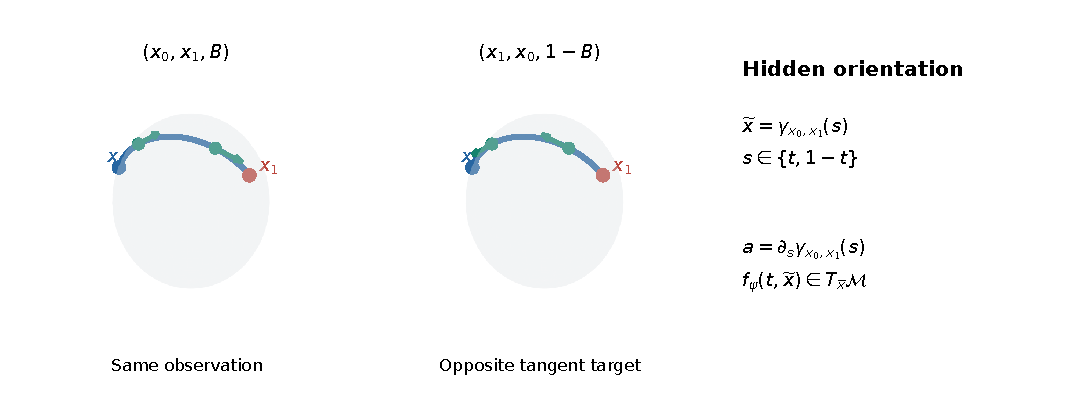
\includegraphics[width=\textwidth]{figures/method_symmetry.pdf}
\caption{\textbf{Geometric midpoint symmetry.} Two potential observations at $t$ and $1-t$ are shown on a sphere geodesic. Swapping endpoints and complementing the hidden flip preserves the selected point and reverses its tangent target. The critic sees $(t,\widetilde x)$, but not the flip or endpoints. These are schematic geometric curves, not experimental samples. At inference, only the constrained generator is used.}
\label{fig:symmetry}
\end{figure*}

Our contribution has three parts. First, we give an intrinsic, time-integrated midpoint discrepancy with a quantitative distributional guarantee and tangent-fiber variational representation. Second, we derive the corresponding one-step generator algorithm and specify its geometric and differentiation requirements. Third, we examine practical learning through initialization/objective controls, completed cells of a modern one-step comparison, and a two-object rigid-grasp pilot. The empirical record does not establish competitive superiority: the modern sweep is incomplete and geometric validity is not physical grasp success. The mesh study uses a projected surrogate rather than an exact spectral path.

\section{Background and Related Work}
\paragraph{Geometric flows and one-step maps.}
Flow Matching regresses a conditional path velocity rather than differentiating a likelihood through a learned ODE \citep{lipman2023flow}; stochastic interpolants provide a broader path-based viewpoint \citep{albergo2023building}. RFM and Riemannian score-based models incorporate manifold geometry into their objectives \citep{debortoli2022riemannian,chen2024general}. Consistency and flow-map approaches already provide one- or few-step manifold generation \citep{cheng2025rcm,davis2026gfm,woo2026rmf,zhong2026rmf}. We do not claim that one-step manifold generation is new. Our specific object is a hidden-flip conditional tangent-moment discrepancy and its variational training rule.

\paragraph{Midpoint and distributional objectives.}
MGM supplies midpoint cancellation and a variational quadratic critic in Euclidean space \citep{shlenskii2026midpoint}; Zero-Flow Encoders also study a zero-field criterion \citep{wang2026zeroflow}. MeanFlow learns average velocities \citep{geng2025mean}, while Drifting Models evolve a generator's output distribution during training \citep{deng2026drifting}. Kernel-Gradient Drifting Models extend kernel-induced fields to manifolds \citep{estebancasadevall2026kgdm}. Our tangent \emph{velocity} target requires its own argument: generalized stochastic MGM can use an endpoint chord, which is not the derivative of a noisy interpolant.

\paragraph{Wasserstein gradient flows.}
These flows decrease an energy on probability measures using optimal transport geometry \citep{jordan1998variational,ambrosio2008gradient}. Kernel discrepancies also admit such dynamics \citep{arbel2019maximum}. Recent one-step work includes W-Flow \citep{han2026wflow}, the Wasserstein interpretation of drifting \citep{gretton2026wasserstein}, RW-Flow on compact manifolds \citep{nurgulan2026rwflow}, and Riemannian Wasserstein gradient-flow models \citep{li2026rwgf}. The existence of these intrinsic one-step methods makes the choice of discrepancy, assumptions for identifiability, and practical objective the relevant comparison. Our theorem does not require a nondegenerate smoothing kernel, but does require full time coverage and true finite-energy path velocities. We distinguish the Riemannian metric on data from a Wasserstein metric on distributions; \cref{sec:wgf} explains why ordinary generator SGD is not automatically the latter's gradient flow.

\section{Geometric Midpoint Learning}
\label{sec:method}
\subsection{Paths, Observations, and Tangent Targets}
Let $(\M,g)$ be a complete, connected, finite-dimensional smooth Riemannian manifold without boundary, with distance $d_g$ and tangent spaces $T_x\M$. Let $\mu,\nu$ have finite first moments. We write $\norm{g_x}{u}^2=g_x(u,u)$. The target is $\nu$ and the generated law is $\mu_\theta=(G_\theta)_\#p_Z$, where $p_Z$ is a fixed latent distribution and $G_\theta(z)\in\M$. The loss endpoint is the generator output, not its latent input.

\begin{assumption}[Admissible reversible paths]
\label[assumption]{ass:paths}
A measurable path kernel assigns to each pair $(x,y)$ a law on absolutely continuous curves $\gamma:[0,1]\to\M$ with endpoints $x,y$. Endpoint exchange sends this law to its time reversal. For independent $X_0\sim\mu$, $X_1\sim\nu$, the resulting path has finite expected action:
\begin{equation}
\mathcal A_\Gamma(\mu,\nu)=\E\int_0^1\norm{g_{\gamma_s}}{\dot\gamma_s}^2\dd s<\infty.
\label{eq:action}
\end{equation}
\end{assumption}

Deterministic reversible paths are a special case. A selected constant-speed minimizing geodesic is
\begin{equation}
\gamma_s=\Exp_{X_0}\big(s\Log_{X_0}(X_1)\big),
\label{eq:geodesic}
\end{equation}
with action $\E d_g(X_0,X_1)^2$. Finite second endpoint moments suffice for this action to be finite. Nonunique geodesics require a measurable reversal-consistent choice; independently selected branches for the two endpoint orders need not meet \cref{ass:paths}.

Draw $t\sim\mathcal U(0,1/2)$ and $B\sim\mathrm{Bernoulli}(1/2)$ independently of endpoints and path randomness. Set
\begin{equation}
s=t+B(1-2t),\quad \widetilde X_t=\gamma_s,\quad A_t=\dot\gamma_s.
\label{eq:flip}
\end{equation}
Here $A_t$ is the derivative in \emph{path time} $s$, not the derivative of $\gamma_{s(t)}$ in $t$. The flip is hidden from the critic. With $\bar\rho_t=\Law(\widetilde X_t)$, define
\begin{equation}
m_t(x)=\E[A_t\mid \widetilde X_t=x,t]\in T_x\M.
\label{eq:conditional}
\end{equation}
This conditional expectation is fiberwise: after conditioning on $x$, every target belongs to the same inner-product space $T_x\M$. No identification of different tangent spaces is needed.

\subsection{A Definite Intrinsic Discrepancy}
\begin{definition}[Geometric midpoint discrepancy]
\label[definition]{def:divergence}
Using the normalized uniform time law, define
\begin{equation}
\D_\Gamma^g(\mu,\nu)
=\E_{t\sim\mathcal U(0,1/2)}\E_{\bar\rho_t}\norm{g_x}{m_t(x)}^2.
\label{eq:divergence}
\end{equation}
This equals twice the integral over $[0,1/2]$.
\end{definition}

\begin{theorem}[Definiteness and transport control]
\label{thm:divergence}
Under \cref{ass:paths}, $\D_\Gamma^g$ is symmetric and nonnegative, and
\begin{equation}
W_1(\mu,\nu)^2\leq\D_\Gamma^g(\mu,\nu)\leq\mathcal A_\Gamma(\mu,\nu).
\label{eq:bounds}
\end{equation}
Moreover, $\D_\Gamma^g(\mu,\nu)=0$ if and only if $\mu=\nu$. Here $W_1$ uses $d_g$. For constant-speed minimizing geodesics the upper bound is $\E_{\mu\otimes\nu}d_g(X_0,X_1)^2$.
\end{theorem}

\paragraph{Proof idea.}
When $\mu=\nu$, endpoint exchange and path reversal preserve $\widetilde X_t$ and negate $A_t$ (\cref{fig:symmetry}); thus $m_t=0$. For a smooth $1$-Lipschitz function $\varphi$, the chain rule and folding time give
\begin{align}
\E_\nu\varphi-\E_\mu\varphi
&=\E\int_0^1 g_{\gamma_s}(\grad\varphi,\dot\gamma_s)\dd s\notag\\
&=\E_t\E_{\bar\rho_t}g_x(\grad\varphi(x),m_t(x)).
\label{eq:fundamental}
\end{align}
Cauchy--Schwarz bounds its absolute value by $\sqrt{\D_\Gamma^g}$. Kantorovich--Rubinstein duality gives the lower bound; conditional Jensen gives the upper bound. The complete density-free proof is in \cref{app:proofs}. Time integration and the \emph{actual} path derivative are essential. Cancellation at a single midpoint does not establish \cref{eq:fundamental}.

\subsection{Variational Objective and Generator Updates}
Let $f_t(x)\in T_x\M$ be square-integrable under the time-observation law. Completing the square in each fiber gives the following representation.
\begin{proposition}[Tangent variational representation]
\label[proposition]{prop:variational}
For every such $f$,
\begin{align}
\Lcal(\mu,\nu;f)
&=\E\big[2g_{\widetilde X_t}(f_t(\widetilde X_t),A_t)
-\norm{g_{\widetilde X_t}}{f_t(\widetilde X_t)}^2\big]\notag\\
&=\D_\Gamma^g(\mu,\nu)
-\E\norm{g_{\widetilde X_t}}{f_t(\widetilde X_t)-m_t(\widetilde X_t)}^2.
\label{eq:variational}
\end{align}
Consequently $\sup_f\Lcal=\D_\Gamma^g$, attained at $f=m$.
\end{proposition}

Riemannian MGM (\RMGM, ours) parameterizes a manifold-valued generator $G_\theta$ and tangent critic $f_\psi$ in
\begin{equation}
\min_\theta\max_\psi\;\Lcal(\mu_\theta,\nu;f_\psi).
\label{eq:saddle}
\end{equation}
The critic equivalently minimizes tangent regression,
\begin{equation}
\Lcal_C=\E\norm{g_{\widetilde X_t}}{f_\psi(t,\widetilde X_t)-A_t}^2,
\label{eq:critic}
\end{equation}
since $\E\norm{g_{\widetilde X_t}}{A_t}^2$ is constant in $\psi$. This term is \emph{not} constant in $\theta$: minimizing critic regression over the generator would change the objective. The generator freezes critic parameters and differentiates both terms in \cref{eq:variational}, including the observation, velocity, and position-dependent metric. \Cref{alg:rmgm} states the procedure.

\begin{algorithm}[t]
\caption{Riemannian Midpoint Generative Models (ours)}
\label{alg:rmgm}
\begin{algorithmic}[1]
\REQUIRE $G_\theta:\mathcal Z\to\M$, tangent critic $f_\psi$, path kernel $\Gamma$, data sampler $\nu$
\FOR{each outer training iteration}
\STATE Draw $z\sim p_Z$, $x_1\sim\nu$, $t\sim\mathcal U(0,1/2)$, $B\sim\mathrm{Bernoulli}(1/2)$.
\STATE $x_0\gets G_\theta(z)$; $s\gets t+B(1-2t)$.
\STATE Sample path; evaluate $\widetilde x=\gamma_s$ and $a=\partial_s\gamma_s$.
\STATE Detach generator outputs; descend \cref{eq:critic} in $\psi$.
\STATE Draw a fresh batch and recompute $(\widetilde x,a)$.
\STATE Freeze $\psi$; descend \cref{eq:variational} in $\theta$ through all geometry-dependent terms.
\ENDFOR
\STATE \textbf{Return} $G_\theta$; sample with $z\sim p_Z$, $x=G_\theta(z)$.
\end{algorithmic}
\end{algorithm}

The proposition concerns an unrestricted population critic. A neural critic gives a lower bound with an approximation gap; its empirical value can be negative and is not a certified upper bound on $W_1$. Existence of a zero population optimum also does not imply convergence of alternating neural optimization. We therefore evaluate independent sample discrepancies rather than treating a small training loss as a certificate.

The implementation divides both training losses by the coordinate representation width $q$ (for example, $q=3$ on $\mathbb S^2$). This positive scaling preserves the population optimizer but changes gradient magnitudes. The theorem uses the unscaled discrepancy; for $\D_{\mathrm{impl}}=\D_\Gamma^g/q$ its bound is $W_1^2\leq q\D_{\mathrm{impl}}$.

\paragraph{Gradient contract.}
The path theorem requires only measurability in the endpoints and absolute continuity in path time. Pathwise generator differentiation in \cref{alg:rmgm} requires more: a reparameterization $\gamma_s=F_s(G_\theta(z),X_1,\xi)$ with parameter-independent base noise, endpoint derivatives for the observation and velocity, and conditions permitting differentiation under expectation. Local smoothness with an integrable domination of the corresponding difference quotients is one sufficient condition. Endpoint-dependent discrete path choices instead require their missing score-function terms or another justified gradient estimator. Branchwise automatic differentiation alone does not establish unbiased gradients of the population objective across changing cut-locus or projection branches. The executed losses use such branchwise derivatives, without a general unbiased-gradient claim for these global branch changes. The discrepancy theorem is unaffected by this optimization qualification.

\subsection{Computation and the Two Meanings of Flow}
\label{sec:wgf}
On closed-form geometries, the path and velocity can be evaluated at a sampled time, analytically or with a Jacobian-vector product. The deterministic construction requires no ODE, divergence estimate, or diffusion trajectory. At inference the critic and interpolant are discarded. One neural evaluation still has a geometric cost: projections or factorizations belong in sampling latency.

Interpolation time $s$ defines a loss between two fixed laws; it differs from generator optimization time. A Wasserstein gradient flow decreases an energy $\mathcal E$ through a measure-valued trajectory, formally satisfying
\begin{equation}
\partial_\tau\mu_\tau
=\operatorname{div}_g\left(\mu_\tau\grad_g\frac{\delta\mathcal E}{\delta\mu}(\mu_\tau)\right)
\label{eq:wgf}
\end{equation}
when the first variation and transport chain rule exist. One may investigate $\mathcal E(\mu)=\D_\Gamma^g(\mu,\nu)$ in this framework. Our finite-parameter minimax algorithm establishes neither that first-variation formula nor convergence to \cref{eq:wgf}. Its distinction from kernel and Sinkhorn methods is its specified discrepancy and training construction, not an incompatibility with Wasserstein dynamics. The critic $m_t$ is also not the transport velocity of $\bar\rho_t$: the latter uses the signed target $(1-2B)A_t$.

\section{Geometries and Output Constraints}
\label{sec:geometries}
The loss requires an admissible path and tangent critic; the generator separately enforces output validity. \Cref{tab:geometries} summarizes the main cases. An admissible path family transfers \cref{thm:divergence} independently of the architecture used to realize the endpoint law.

\begin{table*}[t]
\caption{\textbf{Geometric realizations of \RMGM\ (ours).} Closed-form entries allow simulation-free deterministic interpolation. Numerical floors restrict or approximate the ideal domain. General mesh paths may need numerical solution; the mesh experiments use a separate surrogate.}
\label{tab:geometries}
\centering
\small
\begin{tabular}{@{}llll@{}}
\toprule
Domain & Generator constraint & Path and critic metric & Numerical issue \\
\midrule
Sphere $\mathbb S^{d-1}$ & Normalize nonzero output & Great-circle arc; tangent dot product & Near-antipodal pairs \\
Flat torus $\mathbb T^d$ & Angles modulo $2\pi$ & Shortest periodic displacement; flat metric & Ties at angle $\pi$ \\
Hyperbolic ball & Radial map inside the ball & Hyperbolic geodesic; conformal metric & Boundary conditioning \\
SPD matrices & Cholesky factor $LL^\top+\varepsilon I$ & Affine-invariant geodesic and metric & Spectral derivatives \\
Triangular surface & Projection or chart map & Admissible surface path required & Continuity and coverage \\
\bottomrule
\end{tabular}
\end{table*}

\paragraph{Spheres and flat tori.}
For the unit sphere, $G_\theta(z)=h_\theta(z)/\|h_\theta(z)\|_2$ and $f_\psi(t,x)=(I-xx^\top)h_\psi(t,x)$. The loss uses the great-circle path away from antipodes. On a flat torus, write $\delta=\operatorname{wrap}_{(-\pi,\pi]}(x_1-x_0)$. Then $\gamma_s=(x_0+s\delta)\bmod 2\pi$ and $A_s=\delta$, with a reversal-consistent tie convention. The earlier controlled critics and fields consume raw wrapped angles and can have seam effects. The newer one-step protocol instead uses periodic spatial features and an unfitted uniform-base residual generator. These are distinct experimental architectures, not interchangeable checkpoints.

\paragraph{Rigid poses.}
For the grasp pilot we represent SE(3) as the product manifold $SO(3)\times\R^3$, with product geodesics and a product metric after mesh-based translation normalization. The output rotation is constrained to $SO(3)$ and the critic has rotational and translational tangent components. This does not assert a bi-invariant metric on the rigid-motion group. The product geodesic and its true velocity give simulation-free targets away from the rotation cut locus; the finite-network and collision limitations remain separate.

\paragraph{Hyperbolic space and SPD matrices.}
On the Poincar\'e ball, the metric is conformally Euclidean; the local factor must enter the loss and generator gradient. For $X\in\mathbb S_{++}^n$, affine-invariant choices are
\begin{align}
g_X(U,V)&=\Tr(X^{-1}UX^{-1}V),\notag\\
\gamma_s&=X_0^{1/2}(X_0^{-1/2}X_1X_0^{-1/2})^sX_0^{1/2}.
\label{eq:spd}
\end{align}
The critic is symmetric, with the metric computed through whitened tangent matrices. A log-Euclidean alternative \citep{arsigny2006log} reduces to Euclidean MGM in matrix-logarithm coordinates; it changes the metric and is not equivalent to the affine-invariant experiment. \Cref{app:geometry} gives numerical qualifications.

\paragraph{Directed paths and surfaces.}
An RFM premetric path need not be reversible. Mixing a directed kernel $K_{x,y}$ with the reversed kernel $K_{y,x}$, with equal weights, creates a reversible kernel (\cref{prop:symmetrize}). This provides a general-geometry construction but retains numerical integration and differentiation costs.

Our exploratory mesh implementation instead uses
\begin{equation}
\widetilde x=\Pi_\M((1-s)x_0+sx_1),\qquad
a=\Pi_{T_{\widetilde x}\M}(x_1-x_0).
\label{eq:mesh-surrogate}
\end{equation}
In a region projecting to a fixed face interior, this is a useful local construction. Across nearest-face switches the path can jump, and its assigned tangent need not represent the full current. Thus \cref{thm:divergence} is not applied to these runs. Similarly, a radial sphere-to-mesh map produces surface points but need not be bijective or cover concave patches. Topological equivalence to a sphere does not justify that particular map. These are empirical parameterization studies, not an exact spectral-path implementation.

\section{Experiments}
\label{sec:experiments}
We distinguish three evidence blocks: a completed nine-task initialization/objective study, a paused comparison with recent one-step methods, and a completed two-object grasp pilot. None is an original-author-budget RFM reproduction. All numerical claims below use completed runs; interrupted checkpoints appear only in validation diagnostics.

\subsection{Data and Metrics}
Four Earth-event datasets lie on $\mathbb S^2$ (Volcano, Earthquake, Flood, Fire); four protein-angle datasets lie on $\mathbb T^2$ (General, Glycine, Proline, Pre-Pro); RNA uses $\mathbb T^7$. Data follow the RFM pipeline and share a fixed 80/10/10 row split. The local RNA preprocessing has 9,473 rows. These historically inspected splits do not test unseen proteins, temporal forecasting, or independent source groups.

For these nine tasks the primary score is the biased squared MMD V-statistic with $k(x,y)=\exp(-\|e(x)-e(y)\|_2^2/h^2)$, using the identity sphere embedding or circular torus embedding. The bandwidth is fixed from training data. Up to 1,024 held-out points are shared across models; generated batches have the same size. We average three draws within each training seed and report mean and sample SD over seeds 0, 1, 2. The finite-sample biased score need not vanish under the correct law. Intrinsic nearest-neighbor, coverage, 1-NNA, and constraint metrics complement MMD. Exact NLL is unavailable for these implicit generators; sample scores do not reproduce published likelihood tables.

\subsection{Initialization and Objective Controls}
The earlier controlled study uses batch 256, width-128 networks, and AdamW learning rate $2\times10^{-4}$ with no weight decay. Midpoint models take 2,000 outer iterations, each with one critic and one generator update. The smaller controlled RFM runs for 2,000 or 10,000 updates and samples with 128 field calls. These are iteration comparisons, not matched optimizer work or FLOPs. No validation/test checkpoint selection is used in this block.

\begin{table*}[t]
\caption{\textbf{Controlled real-data sample quality.} Biased $\widehat{\mathrm{MMD}}^2\times10^3$ (lower is better), mean $\pm$ sample SD over three training seeds, after averaging three draws per seed. Mixture initialization uses training data only. RFM uses 128 field calls at inference. Budgets are updates/outer iterations, not equal FLOPs; the smaller controlled RFM is not the original author-budget model.}
\label{tab:main}
\centering\small
\begin{tabular}{@{}lrrrrr@{}}
\toprule
Dataset & Test $n$ & Mixture init. & R-MGM mixture (ours) & RFM & RFM (longer) \\
 & & 0 updates & 2,000 iterations & 2,000 updates & 10,000 updates \\
\midrule
Volcano & 82 & $16.20\,\pm\,5.24$ & $13.91\,\pm\,4.89$ & $15.04\,\pm\,1.07$ & $12.86\,\pm\,0.31$ \\
Earthquake & 612 & $1.73\,\pm\,0.65$ & $1.76\,\pm\,0.61$ & $6.17\,\pm\,0.38$ & $3.83\,\pm\,0.32$ \\
Flood & 487 & $1.68\,\pm\,0.51$ & $1.61\,\pm\,0.12$ & $4.04\,\pm\,0.31$ & $2.26\,\pm\,0.39$ \\
Fire & 1024 & $0.73\,\pm\,0.59$ & $1.01\,\pm\,0.58$ & $4.06\,\pm\,0.52$ & $0.91\,\pm\,0.13$ \\
General & 1024 & $0.61\,\pm\,0.06$ & $33.75\,\pm\,3.94$ & $40.69\,\pm\,0.77$ & $23.25\,\pm\,2.20$ \\
Glycine & 1024 & $0.90\,\pm\,0.32$ & $14.29\,\pm\,2.46$ & $18.58\,\pm\,0.88$ & $6.73\,\pm\,0.43$ \\
Proline & 763 & $0.89\,\pm\,0.53$ & $88.86\,\pm\,3.13$ & $94.25\,\pm\,2.35$ & $20.97\,\pm\,1.93$ \\
Pre-Pro & 691 & $1.42\,\pm\,0.35$ & $16.84\,\pm\,15.62$ & $36.64\,\pm\,1.32$ & $17.33\,\pm\,2.21$ \\
RNA (7D) & 947 & $1.52\,\pm\,0.10$ & $2.37\,\pm\,0.20$ & $205.44\,\pm\,1.84$ & $101.07\,\pm\,4.20$ \\
\bottomrule
\end{tabular}
\end{table*}

Table~\ref{tab:main} reports fixed-checkpoint outcomes. Across the 9 fully evaluated tasks, midpoint-trained mixtures have lower mean MMD than their initialization on 2, the 2,000-update flow on 9, and the longer 10,000-update flow on 4. These are descriptive counts, not significance tests or a ranking against author-budget models. Training worsens the mean initialization score on 7 tasks at these settings. The initialization column attributes fit present before training to the restricted mixture model. The degradations expose failures of the implemented finite-critic training procedure, but do not isolate a unique cause or support universal improvement. Figure~\ref{fig:controlled} shows fixed-seed sample visualizations; full-dimensional numerical evaluation is retained for RNA. The matched MMD-trained MLP has lower mean MMD than the midpoint-trained MLP on 3 of 3 representative tasks (Table~\ref{tab:ablation}); these runs do not establish an advantage of the midpoint objective over this direct loss. It also has lower mean nearest-neighbor distance on 3 and higher coverage on 3 of these tasks (supplemental Table~\ref{tab:mlp-metrics}), without implying a universal objective ranking.

\begin{table}[t]
\caption{\textbf{Initialization and objective controls.} Biased MMD$^2\times10^3$, mean $\pm$ SD across three training seeds. All trained rows use 2,000 iterations/updates. MLP rows share architecture and output constraints; mixture rows have a different restricted parameterization.}
\label{tab:ablation}
\centering\small
\setlength{\tabcolsep}{4pt}
\begin{tabular}{@{}lrrr@{}}
\toprule
Method & Fire & General & RNA \\
\midrule
Init. GMM & $0.7\,\pm\,0.6$ & $0.6\,\pm\,0.1$ & $1.5\,\pm\,0.1$ \\
R-MGM GMM & $1.0\,\pm\,0.6$ & $33.8\,\pm\,3.9$ & $2.4\,\pm\,0.2$ \\
R-MGM MLP & $21.4\,\pm\,16.4$ & $60.7\,\pm\,10.8$ & $283.0\,\pm\,119.0$ \\
MMD MLP & $2.2\,\pm\,0.7$ & $31.1\,\pm\,0.8$ & $8.5\,\pm\,0.7$ \\
RFM (1) & $27.5\,\pm\,2.3$ & $61.0\,\pm\,1.5$ & $343.6\,\pm\,4.6$ \\
RFM (128) & $4.1\,\pm\,0.5$ & $40.7\,\pm\,0.8$ & $205.4\,\pm\,1.8$ \\
\bottomrule
\end{tabular}
\end{table}




The mixture starts from train-fitted centers, scales, and weights; only centers and scales receive pathwise midpoint gradients. Hard component boundaries leave weights fixed. Matched random-MLP midpoint and direct-MMD controls isolate objective choice on three tasks. The direct-MMD control is not KGDM or RW-Flow. These results expose substantial optimization failures rather than a general efficacy claim. Post hoc, single-seed validation diagnostics examine periodic features, critic warmup, extra critic steps, and a true-velocity randomized torus path (\cref{app:stability}); they do not alter this table.

\subsection{Recent One-Step Comparisons: Completed Cells}
\label{sec:recent}
We implement RW-Flow-C \citep{nurgulan2026rwflow}, KGDM \citep{estebancasadevall2026kgdm}, and the RMF-MT variant of \citet{zhong2026rmf}. This is the latter MeanFlow construction, not the distinct method of \citet{woo2026rmf}. Midpoint, RW-Flow-C, and KGDM share an unfitted, uniform-prior point generator with width 128, three affine layers, and 16 latent dimensions. RMF retains its source-derived two-time network, with a different parameter count. Every sampler uses one neural evaluation. Method-source fidelity and adaptations are detailed in \cref{app:recent-protocol}.

Configurations are selected on representative validation tasks and frozen before final tests. Completed jobs use 50,000 generator/field updates, batch 256, and validation-selected checkpoints, including initialization. MGM additionally uses 500 critic warmup updates and five or ten critic updates per generator update. Critic refinement, tuning grids, model parameters, and compute are not matched.

\begin{table*}[t]
\centering\small
\caption{\textbf{Completed modern one-step comparisons.} Test $\widehat{\mathrm{MMD}}_V^2\times10^3$, mean $\pm$ training-seed SD (three seeds); lower is better. Each available cell completed 50,000 generator/field updates and uses a validation-selected checkpoint. All samplers use one network evaluation. The paused 108-job plan has only 18 completed jobs; n/a means unavailable, not a performance score. These are small-network adaptations, not original-author benchmark reproductions.}
\label{tab:recent}
\begin{tabular}{@{}llrrrr@{}}
\toprule
Dataset & Test $n$ & R-MGM (ours) & RW-Flow-C & KGDM & RMF-MT \\
\midrule
Volcano & 82 & $13.135\,\pm\,1.555$ & $12.537\,\pm\,0.277$ & $13.900\,\pm\,1.694$ & $11.957\,\pm\,0.275$ \\
Earthquake & 612 & n/a & n/a & $2.132\,\pm\,0.115$ & $2.814\,\pm\,0.694$ \\
\bottomrule
\end{tabular}
\end{table*}

\Cref{tab:recent} reports the completed cells of the nine-task, four-method, three-seed plan: 18 of 108 jobs at this snapshot. Only Volcano supports a completed four-method comparison. Its smallest observed mean is RMF-MT's; MGM does not outperform it, and no significance claim is made. Earthquake has only KGDM and RMF-MT completed across all seeds; its two interrupted MGM runs have no test results. Remaining tasks are unavailable, not negative scores. \Cref{fig:recent-volcano} shows fixed seed-0 samples; recorded validation curves appear in \cref{fig:recent-curves}. A 50,000-update cap does not certify convergence. Training shared one GPU between at most two workers; isolated latency profiling was not run, so this block supplies no inference-speed or training-efficiency ranking.

\begin{figure*}[t]
\centering
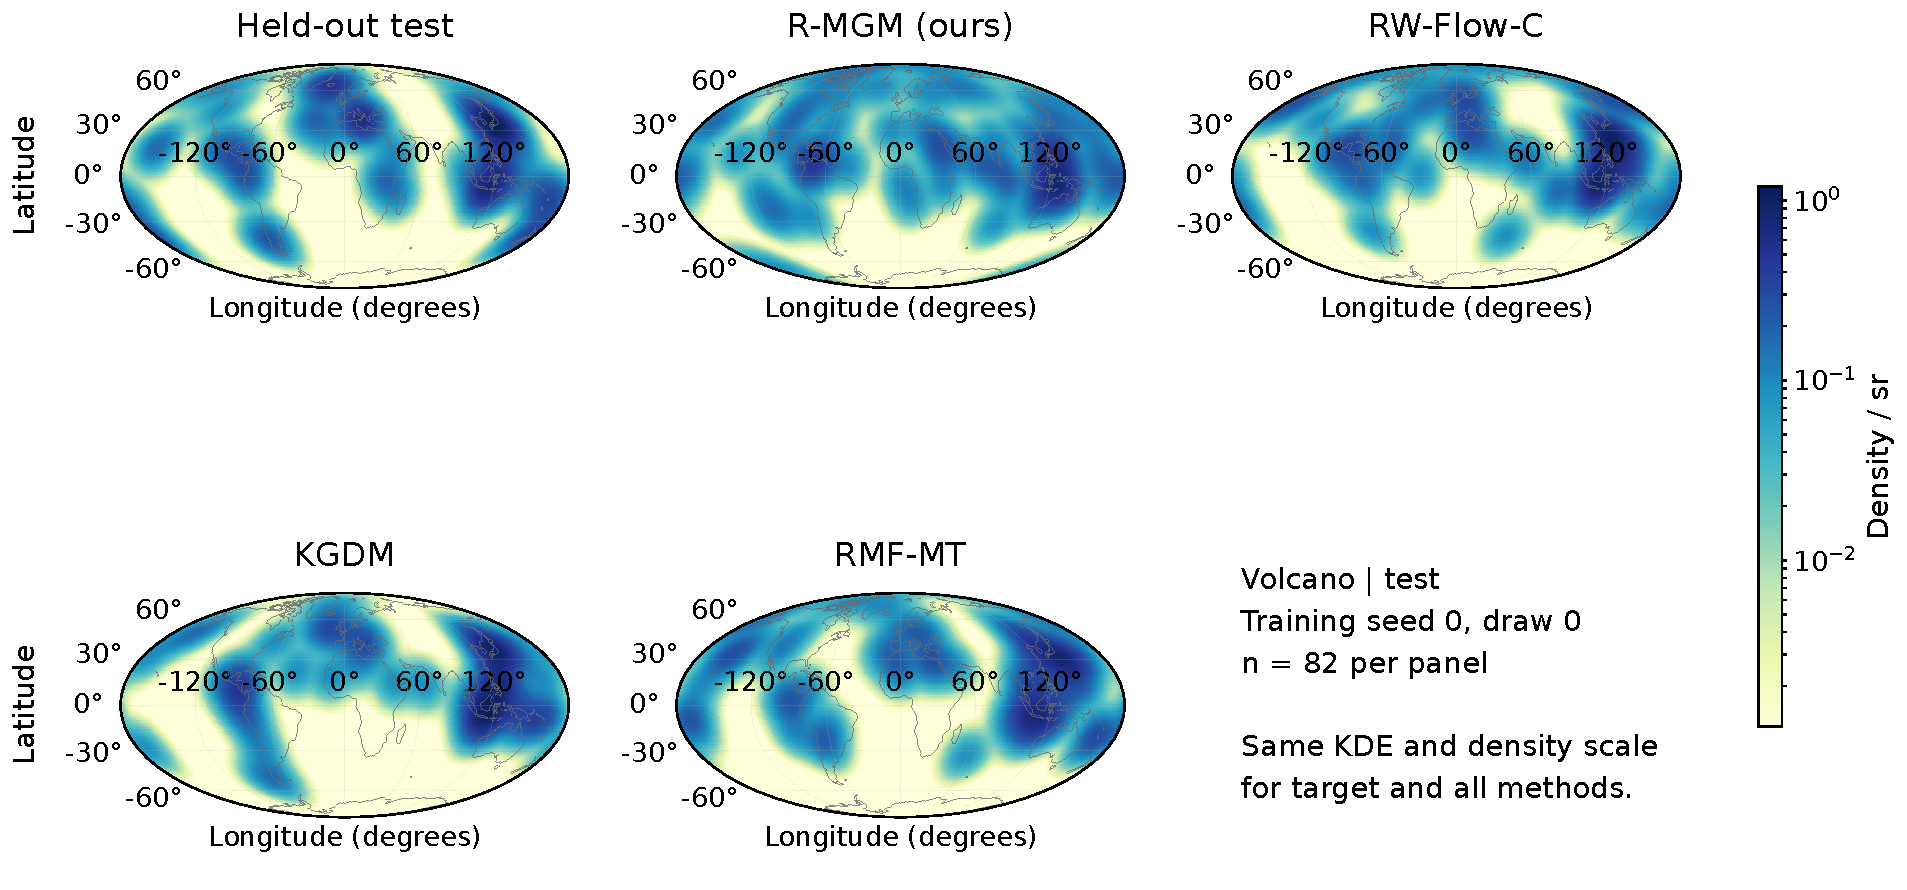
\includegraphics[width=.94\textwidth]{figures/recent_volcano.pdf}
\caption{\textbf{Completed one-step comparison on Volcano.} Fixed test target and training seed 0, generated draw 0; $n=82$ per panel. Checkpoints are validation-selected after each run completed 50,000 updates. All panels use the same spherical KDE and logarithmic density scale. These are sample densities, not likelihoods or additional independent training seeds. Quantitative means use all three seeds in \cref{tab:recent}.}
\label{fig:recent-volcano}
\end{figure*}

\subsection{SE(3) Grasp Proposals}
\label{sec:grasp}
We use the two public, matched Mug/Table HDF5 and mesh examples from ACRONYM \citep{eppner2021acronym}. Positive source poses are split 80/10/10 within each known object; this is not full ACRONYM or unseen-object transfer. The product $SO(3)\times\R^3$ geometry constrains rotations and normalizes translation from mesh bounds. Each of MGM, local RFM, and a source-loss RMF-MT adaptation completes 10,000 generator/field updates for three seeds. No validation/test tuning or checkpoint selection is used; MGM adds 100 warmup and 50,000 critic updates per seed. RFM uses 50 or 100 inference evaluations, while MGM and RMF-MT use one. Architecture and path adaptations preclude an original-author grasp reproduction.

\begin{table*}[t]
\centering\small
\caption{\textbf{Completed two-object SE(3) pilot.} Equal object means are formed within each training seed, then mean $\pm$ sample SD over three seeds. Every model trains for 10,000 generator/field updates. Pose MMD is an \emph{unbiased product-kernel} statistic, distinct from \cref{tab:main,tab:recent}. The thin-gripper static proxy is not physical success; full-Franka collision tests a different geometry. Reference poses have 92\%/100\% static-proxy passes on Mug/Table and 0\% full collisions. Lower pose MMD and collision, but higher proxy fraction, are better.}
\label{tab:grasp}
\begin{tabular}{@{}lrrrr@{}}
\toprule
Method & NFE & Pose MMD$^2\times10^3$ & Static proxy (\%) & Full collision (\%) \\
\midrule
R-MGM (ours) & 1 & $4.265\,\pm\,1.591$ & $24.67\,\pm\,1.76$ & $71.00\,\pm\,5.22$ \\
RMF-MT adaptation & 1 & $12.096\,\pm\,1.458$ & $10.83\,\pm\,2.47$ & $34.17\,\pm\,0.29$ \\
RFM & 50 & $0.530\,\pm\,0.099$ & $32.17\,\pm\,3.51$ & $67.00\,\pm\,2.50$ \\
RFM & 100 & $0.515\,\pm\,0.119$ & $32.00\,\pm\,3.28$ & $66.67\,\pm\,2.25$ \\
\bottomrule
\end{tabular}
\end{table*}

\Cref{tab:grasp} averages the two object scores within each seed before computing seed SD. Pose MMD is an unbiased chordal-product-kernel statistic and is not numerically comparable with the sphere/torus score. Static geometric checks use 100 unfiltered draws per object; distribution metrics use 512 generated poses. MGM has lower pose MMD and higher thin-gripper static-proxy fraction than this one-step RMF-MT adaptation, but multi-step RFM is more accurate in pose MMD. MGM's $71.00\%$ mean full-Franka collision rate remains unresolved. Lower collision alone can also reward proposals that miss the object. No finger closure, friction, lifting, scene collision, or reachability is simulated; physical success is unmeasured. \Cref{fig:grasp-current,app:grasp-protocol} give the fixed-sample visualization and protocol.

\subsection{Other Geometries and Numerical Checks}
Float64 endpoint, reversal, and numerical derivative checks on sphere, torus, SPD, and an approximate hyperbolic branch verify implementation conventions, not every floating-point trajectory. Earlier sampling-cost measurements apply only to their recorded architectures and are retained in \cref{app:additional}. On Bunny/Spot targets $k=10,50,100$, historical one-seed, fixed-step-800 runs compare projected mixtures and sphere-map parameterizations. They use the local projected-chord surrogate of \cref{eq:mesh-surrogate}, outside the exact-path theorem; they do not reproduce intrinsic mesh likelihoods. Full figures, controls, and benchmark-coverage limits remain in \cref{app:additional,app:inventory}.

\section{Discussion and Limitations}
The construction supplies a distribution-level justification for a geometric midpoint loss and a direct generator algorithm. Its guarantee requires finite-energy admissible paths and actual path velocities. It does not assert a triangle inequality for $\sqrt{\D_\Gamma^g}$, convergence of finite neural optimization, or universal approximation for a chosen constrained architecture. The transport bound concerns the population critic optimum and does not certify its empirical training loss.

The experimental scope also matters. A smaller flow baseline does not reproduce author-budget RFM, and sample discrepancies cannot be compared with published NLL tables. Objective controls expose substantial optimization failures: good initialized mixtures can degrade and a matched direct-MMD MLP is stronger at the studied setting. Its evaluation-aligned kernel is itself an advantage, not evidence of universal MMD superiority. The modern comparison has only one completed four-method task, where MGM does not lead. The two-object grasp pilot improves on an adapted one-step MeanFlow in pose MMD but not on multi-step RFM; substantial collisions preclude a physical-utility claim. Extra critic work, unequal tuning, small models, and historical row splits limit generalization of these rankings. The mesh surrogate, radial maps, finite-difference targets, and global path-selection gradients need further analysis. Real large EEG covariance experiments and the remaining modern-comparison cells are not completed.

\section{Conclusion}
Riemannian midpoint learning supplies an intrinsic distribution discrepancy and a direct generator training rule. The population criterion identifies endpoint laws and controls Wasserstein-1 distance, with simulation-free closed-form interpolation where available. Completed controls, partial modern comparisons, and the rigid-pose pilot do not establish general practical superiority. Initialization, finite critics, gradient estimation, and downstream feasibility remain consequential. These distinctions make both the theoretical guarantee and the present empirical limitations explicit.

\clearpage
\section*{Impact Statement}
This work studies distribution learning on geometric domains. Potential applications include molecular representations, covariance modeling, spatial data, and robot grasp proposals. Geometric validity alone does not establish physical, biological, or clinical validity. The empirical study makes no claim of forecasting hazards, supporting medical decisions, or safely executing grasps. The grasp pilot measures distributional and static geometric properties, not closing, lifting, friction, scene safety, or robot reachability. We use public research datasets and disclose evaluation and licensing limits.
\bibliography{references}
\bibliographystyle{icml2026}
\clearpage
\appendix
\onecolumn
\section{Proofs and Scope of the Guarantees}
\label{app:proofs}
\subsection{Measure-Theoretic Setup}
Let $AC^2([0,1];\M)$ denote absolutely continuous curves with square-integrable metric speed. The kernel in \cref{ass:paths} is measurable on continuous curves with their Borel sigma algebra and concentrated on $AC^2$. Let $\eta_{\mu,\nu}$ be its mixture under $\mu\otimes\nu$. We use a measurable version of the almost-everywhere tangent derivative under $\eta_{\mu,\nu}\otimes\dd s$; changing it on a product-null set does not change the discrepancy. Conditional tangent expectations can be constructed in measurable local orthonormal frames. Orthogonal changes of frame commute with conditional expectation, yielding an intrinsic field. Finite expected action gives square integrability under the folded time-observation law by Tonelli's theorem.

Write $R\gamma(s)=\gamma(1-s)$. Reversibility means $K_{y,x}=R_\#K_{x,y}$; its tangent version satisfies $(R\gamma)'(s)=-\dot\gamma(1-s)$ almost everywhere. Equality in law suffices. No globally smooth, unique logarithm is assumed.

\subsection{Proof of Theorem~\ref{thm:divergence}}
\begin{proof}
\emph{Finiteness and upper bound.} The normalized time density and equal-probability flip give
\begin{align}
\E_{t,B,\eta}\norm{g_{\gamma_s}}{\dot\gamma_s}^2
&=\int_0^{1/2}\E_\eta\big[\norm{g_{\gamma_t}}{\dot\gamma_t}^2
+\norm{g_{\gamma_{1-t}}}{\dot\gamma_{1-t}}^2\big]\dd t\notag\\
&=\E_\eta\int_0^1\norm{g_{\gamma_s}}{\dot\gamma_s}^2\dd s
=\mathcal A_\Gamma(\mu,\nu).
\end{align}
Conditional Jensen in each tangent fiber yields $0\leq\D_\Gamma^g\leq\mathcal A_\Gamma$.

\emph{Symmetry.} Swapping endpoints replaces the path law by its reversal. The transformation $(\gamma,B)\mapsto(R\gamma,1-B)$ preserves the selected point and negates its forward tangent velocity. Thus the observation law under $(\nu,\mu)$ is the same as under $(\mu,\nu)$, with conditional field $-m_t$. Its squared norm has the same expectation.

\emph{Zero on the diagonal.} If $\mu=\nu$, independent endpoints are exchangeable. The preceding transformation preserves the joint law of time and observation while negating $A_t$. Pairing against any bounded measurable tangent test field gives $\E g(h,A_t)=-\E g(h,A_t)=0$. Therefore $m_t=0$ almost everywhere and $\D_\Gamma^g(\mu,\mu)=0$.

\emph{Transport lower bound.} Take a smooth $\varphi$ with $\|\grad\varphi\|_g\leq1$. The chain rule along an absolutely continuous curve gives
\begin{equation}
\varphi(X_1)-\varphi(X_0)=\int_0^1g_{\gamma_s}(\grad\varphi(\gamma_s),\dot\gamma_s)\dd s.
\end{equation}
Finite action implies absolute integrability by Cauchy--Schwarz, justifying Fubini. Folding the interval and conditioning gives \cref{eq:fundamental}. Applying Cauchy--Schwarz under the resulting probability law yields
\begin{align}
\left|\E_\nu\varphi-\E_\mu\varphi\right|
&\leq\big(\E_t\E_{\bar\rho_t}\|\grad\varphi\|_g^2\big)^{1/2}
\sqrt{\D_\Gamma^g}\notag\\
&\leq\sqrt{\D_\Gamma^g}.
\end{align}
For a general $1$-Lipschitz potential, smooth Lipschitz approximation on a separable Riemannian manifold gives a uniform $\epsilon$-approximation with Lipschitz constant at most $1+\epsilon$ \citep{azagra2007smooth}. Apply the preceding estimate and let $\epsilon\downarrow0$. Finite first moments ensure finite endpoint expectations after subtracting a constant. Kantorovich--Rubinstein duality yields $W_1\leq\sqrt{\D_\Gamma^g}$. Since $W_1$ separates finite-first-moment measures, a zero discrepancy implies equal laws. For a constant-speed minimizing geodesic, its pathwise action is $d_g(X_0,X_1)^2$, proving the specialization.
\end{proof}

The lower and upper bounds do not require reversal symmetry. Reversibility supplies symmetry and the zero value on equal laws. Two Dirac endpoints joined by a constant-speed minimizing geodesic attain both bounds, so their constants are sharp. No probability density or global subtraction of endpoints appears in the proof.

\subsection{Continuity-Equation Interpretation}
For any smooth compactly supported vector field $h$, define the tangent current by $J_s(h)=\E_\eta g_{\gamma_s}(h(\gamma_s),\dot\gamma_s)$. Specializing to $h=\grad\varphi$ for smooth compactly supported scalar tests gives the weak equation $\partial_s\rho_s+\operatorname{div}_gJ_s=0$, where $\rho_s=\Law(\gamma_s)$. The folded observation satisfies
\begin{equation}
\bar\rho_t=(\rho_t+\rho_{1-t})/2,\qquad
\bar\rho_t m_t=(J_t+J_{1-t})/2.
\end{equation}
Hence $\partial_t(\rho_t-\rho_{1-t})=-2\operatorname{div}_g(\bar\rho_tm_t)$. If $m_t=0$, this difference is constant. It is zero at $t=1/2$ and equals $\mu-\nu$ at $t=0$, recovering definiteness. The current transporting $\bar\rho_t$ itself is $(J_t-J_{1-t})/2$; the discrepancy field and that transport velocity must not be conflated.

\subsection{Proof of Proposition~\ref{prop:variational}}
\begin{proof}
Conditioning on $(t,\widetilde X_t=x)$ replaces $A_t$ by $m_t(x)$ in the cross term. The identity $2g_x(f,m)-\|f\|_{g_x}^2=\|m\|_{g_x}^2-\|f-m\|_{g_x}^2$ proves the result. Finite action ensures integrability. Taking $f=m$ attains the supremum; a parameterized critic attains it only if it represents that conditional field up to observation-null sets.
\end{proof}

\subsection{Why the Guarantee Is Not a Wasserstein-2 Bound}
For linear paths on an interval $[0,L]$, let
\begin{equation}
\mu_a=\tfrac{1+a}{2}\delta_0+\tfrac{1-a}{2}\delta_L,\quad
\nu_a=\tfrac{1-a}{2}\delta_0+\tfrac{1+a}{2}\delta_L,
\end{equation}
where $a\in(0,1)$. Direct conditioning at the two moving observations gives
\begin{equation}
\D_\Gamma^g=\frac{2a^2L^2}{1+a^2},\qquad
W_1^2=a^2L^2,\qquad W_2^2=aL^2.
\end{equation}
Thus no universal $W_2^2\leq C\D_\Gamma^g$ holds, even on a bounded interval, as illustrated in \cref{fig:bounds}. This Euclidean example specifies the theorem's strength rather than a generation benchmark. On a domain of diameter $R$, $W_2^2\leq R W_1$ instead gives $W_2^2\leq R\sqrt{\D_\Gamma^g}$.

\subsection{Reversible Completion of Directed Paths}
\begin{proposition}
\label[proposition]{prop:symmetrize}
For a measurable finite-energy directed path law $K_{x,y}$ from $x$ to $y$, the kernel
\begin{equation}
\widehat K_{x,y}=\tfrac12K_{x,y}+\tfrac12R_\#K_{y,x}
\end{equation}
is reversible, preserves endpoints, and has action equal to the average of the two directed actions.
\end{proposition}
\begin{proof}
Use the involution $R_\#R_\#K=K$ to obtain $\widehat K_{y,x}=R_\#\widehat K_{x,y}$. Reversal preserves integrated squared speed and swaps endpoints, proving the other assertions.
\end{proof}
A corresponding implementation would sample another hidden orientation bit and use either a forward directed path or the reverse of a backward directed path, with the corresponding derivative sign. This is a construction recipe, not an evaluated branch of the present implementation. It retains the numerical solver's cost and does not supply gradients through a detached solver. A discretization additionally needs endpoint and reversal checks.

\subsection{Time Coverage, Boundaries, and Noise}
A single midpoint need not identify distributions for general reversible paths. On a short arc of $S^1$, connect angles $0$ and $a\in(0,\pi)$ by $\gamma_s=\exp(ia h(s))$, where $h(s)=1/2+4(s-1/2)^3$. This finite-energy path satisfies $h(1-s)=1-h(s)$ but has zero midpoint velocity. Distinct Dirac endpoints therefore have zero midpoint-only discrepancy. This example uses nonconstant speed and does not refute a theorem restricted to constant-speed geodesics.

Endpoint times themselves have zero sampling probability, but the full interval matters: restricting $t$ to $[\epsilon,1/2]$ identifies at most the interior laws $\rho_\epsilon$ and $\rho_{1-\epsilon}$. It does not justify equality of the original endpoints.

For a manifold with boundary, the path proof applies when curves remain inside, are absolutely continuous with finite action, and smooth Lipschitz approximation is valid for the intrinsic length metric. A current proof must hold for tests up to the boundary with no unaccounted source or sink. Interior-only continuity equations or final-output projection do not establish these conditions.

Random differentiable paths are already covered. A noisy interpolant must retain endpoints, reversal symmetry, finite action, and its \emph{full} time derivative. Perturbing a clean point and transporting only its clean velocity can retain cancellation while omitting noise-amplitude and exponential-map derivatives. Thus the deterministic theorem does not establish that noisy surrogate. For numerical targets, define
\begin{equation}
\epsilon^2=\E_{t\sim\mathcal U(0,1/2),B,\eta}\norm{g_{\widetilde X_t}}{\widehat A_t-A_t}^2,
\qquad \widehat m_t(x)=\E[\widehat A_t\mid t,\widetilde X_t=x],
\end{equation}
and $\widehat\D=\E_t\E_{\bar\rho_t}\|\widehat m_t\|_g^2$ under the same normalized law. Conditional Jensen gives $\|\widehat m-m\|_{L^2}\leq\epsilon$, and the triangle inequality implies $W_1\leq\sqrt{\widehat\D}+\epsilon$ for these same admissible observation paths.

\subsection{A Simulation-Free Randomized Torus Path}
\label{app:noisy-torus}
The following construction illustrates a noisy path whose actual derivative is available. On a flat $d$-torus, fix the shortest periodic displacement $\delta$ with a reversal-consistent tie rule. For $\xi\sim\mathcal N(0,I_d)$ independent of endpoints and fixed along the curve, set
\begin{align}
\gamma_s&=(x_0+s\delta+\varepsilon\sin(\pi s)\xi)\bmod2\pi,\notag\\
\dot\gamma_s&=\delta+\varepsilon\pi\cos(\pi s)\xi.
\label{eq:noisy-torus}
\end{align}
Both endpoints are exact. Using the same $\xi$ when reversing endpoints proves pathwise reversal symmetry, since $\sin(\pi(1-s))=\sin(\pi s)$ and the cosine derivative changes sign. Averaging the action over the independent Gaussian removes the cross term and yields
\begin{equation}
\mathcal A_\Gamma(\mu,\nu)=\E\|\delta\|_2^2+\frac{\varepsilon^2\pi^2d}{2}.
\end{equation}
This finite-energy randomized construction falls directly under \cref{thm:divergence}. It uses a differentiable random curve rather than a Brownian trajectory and needs no time-step simulation. Keeping only the clean displacement as target would be a different objective outside this particular proof. A mathematical construction alone does not establish that adding noise improves finite-network training.

\section{Geometric and Numerical Details}
\label{app:geometry}
For unit-sphere endpoints with $\alpha=\arccos(x^\top y)\in(0,\pi)$,
\begin{align}
\Log_x(y)&=\frac{\alpha}{\sin\alpha}(y-\cos\alpha\,x),\\
\Exp_x(v)&=x\cos\|v\|_2+v\frac{\sin\|v\|_2}{\|v\|_2}.
\end{align}
Small-angle limits avoid division by zero. Antipodes require a selected reversible great circle. Clipping an unstable logarithm is a numerical approximation, not a uniqueness result. The periodic displacement tie at $\pi$ on a torus has the same branch issue. Exact ties have probability zero for continuous endpoint laws, but near ties can still degrade numerical accuracy.

The SPD implementation uses the affine-invariant metric in \cref{eq:spd}, with matrix powers and logarithms from symmetric eigendecompositions. Cholesky diagonals are positive and a small jitter raises the spectrum; this fixed floor restricts the family. Log-Euclidean coordinates instead give a globally Euclidean geometry and do not test the affine-invariant metric tensor.

On the curvature-$-1$ Poincar\'e ball, $g_x(u,v)=\lambda_x^2u^\top v$ with $\lambda_x=2/(1-\|x\|_2^2)$. A radial map $0.995\tanh(\|h\|_2)h/\|h\|_2$ stays inside the numerical boundary. The legacy path code uses a central finite difference of radius $10^{-3}$, clamped at endpoint times, for its target velocity. These runs approximate the exact-path construction.

\section{Recent One-Step Comparison: Protocol and Evidence Limits}
\label{app:recent-protocol}

\paragraph{Frozen scope and observed completion.}
The recent comparison is a separate small-network adaptation study, not a
replacement for the earlier controlled suite or a reproduction of the original
papers' full experimental budgets. The frozen \texttt{final\_v1} plan contains
nine datasets, four methods (MGM, KGDM, RW-Flow-C, and RMF-MT), and training
seeds $0,1,2$: $108$ jobs, each allocated $50{,}000$ generator or field updates.
The datasets are Volcano, Earthquake, Flood, and Fire on $\mathbb S^2$;
General, Glycine, Proline, and Pre-Pro on $\mathbb T^2$; and RNA on
$\mathbb T^7$. At the experimental snapshot of October 26, 2026,
\textbf{18/108 jobs were complete, two were interrupted, and 88 had not
started}. Table~\ref{tab:recent-completion} records availability rather than
scores. Only Volcano supports a complete four-method, three-seed comparison;
Earthquake supports three-seed KGDM and RMF-MT results only.

\begin{table}[t]
\caption{Completion at the October 26 pause. C3 denotes three completed
training seeds; I2/N1 denotes two interrupted seeds and one unstarted seed;
N3 denotes three unstarted seeds. Unavailable cells are not performance estimates.}
\label{tab:recent-completion}
\centering\small
\begin{tabular}{@{}p{.39\linewidth}cccc@{}}
\toprule
Dataset & MGM & KGDM & RW-Flow-C & RMF-MT \\
\midrule
Volcano & C3 & C3 & C3 & C3 \\
Earthquake & I2/N1 & C3 & N3 & C3 \\
Flood, Fire, General, Glycine, Proline, Pre-Pro, RNA
 & N3 & N3 & N3 & N3 \\
\bottomrule
\end{tabular}
\end{table}

Earthquake MGM seeds 0 and 1 have durable progress at $40{,}000$ and $20{,}000$
of $50{,}000$ planned updates, respectively; their validation-selected
checkpoints are at $30{,}000$ and $20{,}000$. These are saved progress counts,
not an assertion about the last in-flight update before termination.
\emph{No interrupted-run test results are reported.} Their saved validation
curves and previews remain optimization diagnostics, not completed-test
comparisons. Missing methods or seeds are neither imputed nor treated as
failures. Even on Volcano, MGM does not have the lowest observed mean; the
82-point test set and three training seeds do not establish statistical
significance. No convergence or state-of-the-art claim follows from this pause.

\paragraph{Selection and unequal resources.}
The recipes in \texttt{selected\_config\_v1.json} were selected by fixed-probe
validation kernel MMD on representative Fire, General, and RNA tasks and
transferred within each geometry family. Test scoring was disabled during
calibration and refinement. In final jobs, validation averages three fixed
draws at initialization and every $5{,}000$ updates; the minimum selects the
checkpoint, \emph{including initialization}. A completed job reaches the full
update cap even if its selected checkpoint is earlier. Three test draws are
then evaluated from that checkpoint, without advancing training random-number
streams. This selection protocol does not make the historically exposed row
splits newly blinded or source-group-held-out data.

MGM, KGDM, and RW-Flow-C share a width-128, depth-3 point generator with latent
dimension 16, batch size 256, and generator learning rate $2\times10^{-4}$.
RMF-MT retains a native two-time field network at the same nominal width/depth,
not the common generator. On the sphere these networks have $17{,}411$ and
$51{,}721$ trainable parameters, respectively; the corresponding periodic-torus
counts are $17{,}410$ versus $51{,}718$ in two dimensions and $19{,}335$ versus
$53{,}653$ in seven dimensions. MGM adds a separate critic: ten critic updates
per generator update on the sphere and two-torus, five on the seven-torus,
and 500 critic warmup updates per job. Thus a completed MGM job entails
$500{,}500$ or $250{,}500$ critic updates in addition to generator updates.
The sphere/two-torus refinement uses a width-256 critic without changing the
point generator. Search grids, MGM-specific refinement, optimizer work, and
per-update costs differ across methods. Equal generator/field update caps
therefore do not imply equal tuning effort, model size, or compute.

\Cref{tab:recent-fidelity} summarizes retained constructions and adaptations.
\begin{table}[t]
\caption{Implementation fidelity of the recent comparison. Source-level or
equation-level checks concern implementation, not empirical convergence or
reproduction of published scores.}
\label{tab:recent-fidelity}
\centering\small
\begin{tabular}{@{}p{.12\linewidth}p{.38\linewidth}p{.44\linewidth}@{}}
\toprule
Method & Retained construction & Adaptation or limitation \\
\midrule
MGM & Hidden-flip critic objective with differentiation through observation
and path velocity & Common point generator; extra critic optimization and
validation refinement are separately counted. \\
KGDM & Checksum-pinned released author spherical field
\citep{estebancasadevall2026kgdm} & Common generator and geometry wrapper;
wrapped-log torus extension is an adaptation, not an author torus result. \\
RW-Flow-C & Equation-tested chordal-cost field with independent generated
self banks \citep{nurgulan2026rwflow} & Paper reimplementation, not verified
author code; finite Sinkhorn solves and shared-generator regression. \\
RMF-MT & Zhong et al.'s source-derived loss, two-time network, stopped JVP
target, and PCGrad \citep{zhong2026rmf} & Reduced network/budget and periodic
torus features; distinct from the separate Woo et al. method. \\
\bottomrule
\end{tabular}
\end{table}

\paragraph{Method-specific fidelity.}
KGDM executes the unchanged spherical field from author release revision
\texttt{5860d212}; its source hash is checked before loading. This verified
author release is not asserted to be the original anonymous submission
snapshot. The selected recipe uses its native Gaussian field and step
multiplier 1; the checkpoint's EMA generator supplies the single sampling
evaluation. The torus extension uses wrapped angular logarithms and does not
inherit an unverified convergence or characteristic-kernel guarantee.
RW-Flow-C uses detached transport fields and exponential-map regression
targets, not differentiation through a scalar MMD objective. Its frozen
entropy parameter is $0.3$, flow step $0.2$, and finite Sinkhorn counts are
128/256/1024 for sphere/two-torus/seven-torus. Numerical solver checks do not
turn these finite solves into exact population optimal transport.
RMF-MT is derived from Zhong et al.'s pinned revision \texttt{45d96bcd}, with
native loss/network/JVP/PCGrad equivalence checked against unchanged source
definitions away from geometric singularities. It retains the source's ambient
spherical derivative convention; it is not a new covariant-derivative method.
These controls establish bounded implementation fidelity, not full-original
architecture, schedule, or budget reproduction for any baseline.

\paragraph{Metric and audit boundary.}
The primary sphere/torus score is biased Gaussian embedded-kernel
$\mathrm{MMD}^2$, including within-sample diagonals, with a fixed train-derived
median bandwidth. It is not the minimum matching distance also abbreviated
MMD in some generative-model evaluations. Three draws are averaged within a
training seed before the mean and sample SD across seeds are formed; the SD
does not quantify alternative-split uncertainty. Saved-artifact CPU checks
verify the 18 completed jobs' frozen source/data hashes, update and critic
counts, checkpoint-selection arithmetic, three distinct draws, one sampling
forward, manifold constraints, and an independent NumPy MMD recomputation.
This is a partial-artifact audit, not the full 108-job audit. Training wall
times came from a two-worker contended schedule and are not isolated
per-method speed measurements. The deferred isolated GPU sampling/profile
phase was \emph{not run}; NFE counts are not latency measurements.
\Cref{tab:current-cost} accounts for recorded training in the current
comparison and grasp pilot, separately from the earlier controlled suite.
\begin{table}[H]
\centering\small
\caption{Recorded training on one RTX 4090 (24 GB), PyTorch 2.5.1/CUDA 12.1. Minutes sum per-job training wall times, including critic warmup but excluding validation/evaluation; two concurrent workers cause overlapping wall time, so this is not device occupancy or an efficiency ranking. Partial rows stop at durable checkpoints and omit discarded in-flight updates. These rows exclude calibration/refinement, solver/throughput probes, failed preliminary attempts, and older studies; they are not total project GPU cost. The earlier 72-job controlled bundle separately records 17.03 training minutes.}
\label{tab:current-cost}
\begin{tabular}{@{}lrrrrr@{}}
\toprule
Evidence block & Jobs & G/field updates & Critic updates & Minutes & Max workers \\
\midrule
Recent completed jobs & 18 & 900,000 & 1,501,500 & 163.24 & 2 \\
Recent saved partial jobs & 2 & 60,000 & 601,000 & 18.88 & 2 \\
Completed grasp jobs & 9 & 90,000 & 150,300 & 22.06 & 1 \\
\bottomrule
\end{tabular}
\end{table}

The evidence ledger is \texttt{final\_v1/protocol.json} and the
\texttt{paused\_2026\_10\_26} report, \texttt{job\_status.csv}, and
\texttt{partial\_audit\_manifest.json}, under the comparison artifact root.

\section{Two-Object SE(3) Held-Out-Pose Pilot}
\label{app:grasp-protocol}

\paragraph{Actual data and split provenance.}
The separate completed pilot uses the two public, licensed ACRONYM example
objects Mug and Table, with actual matched meshes and HDF5 grasp poses
\citep{eppner2021acronym}. The assets are pinned to the official release
revision \texttt{d02f58fb}; dataset terms are CC BY-NC 4.0 (repository code is
MIT). No synthetic poses, substitute meshes, or unlicensed additional objects
are included. Each object has 2,000 source poses; 1,290 Mug and 1,559 Table
poses carry positive historical FleX labels. A seed-2026 permutation of these
positive HDF5 source indices gives disjoint within-object 80/10/10 partitions:
Mug has 1,032/129/129 train/validation/test poses, and Table has
1,247/155/157. Exact source indices and asset/cache/split hashes are retained.
Both object geometries are intentionally known in all partitions: this is
\emph{held-out-pose evaluation on two known objects}, not unseen-object
generalization or a full ACRONYM benchmark. Mesh bounds alone define center
and radius normalization; held-out grasp statistics are not used. HDF5
translations are already in meters, so object scale is applied only to meshes.

\paragraph{Training and baseline interpretation.}
All nine jobs (three methods, seeds $0,1,2$) completed exactly $10{,}000$
generator/field updates, followed by 24 validation/test evaluations. Training
samples the two objects uniformly and uses only their training poses. Models
use width 128, batch 256, and Adam learning rate $2\times10^{-4}$. The primary
checkpoint is always the final one: no validation/test early stopping,
hyperparameter, checkpoint, or NFE selection is performed. MGM and RMF-MT
sample in one network evaluation; the same trained RFM field
\citep{chen2024general} is evaluated by exponential Euler at both 50 and 100
evaluations. MGM additionally performs 100 critic warmup updates and five
critic updates per generator update, or $50{,}100$ critic updates per seed.
Consequently the pilot is not optimizer-work- or compute-matched.

The pose geometry is the $\mathrm{SO}(3)\times\mathbb R^3$ product
representation of SE(3), with mesh-normalized translations. RFM is a local
common-architecture geodesic-matching implementation. The pilot's RMF-MT
executes the pinned author's decomposed source loss and PCGrad, but uses a
common PointNet/six-vector architecture, RoMa geodesics, zero endpoint noise,
and declared optimizer/path adaptations. Its data-at-zero, noise-at-one path
is paired with backward sampling; no forced diagonal-time fraction is added.
It is a \emph{source-loss architecture adaptation}, not reproduction of the
author's native SDF-network grasp experiment \citep{zhong2026rmf}.

\paragraph{Distinct distribution metric and aggregation.}
Each method/seed produces 512 poses per object, evaluated against that object's
held-out source poses. With $p$ in mesh-normalized coordinates, the fixed
product kernel is
\begin{equation}
k((R,p),(R',p'))=\frac14\sum_{h\in\{0.5,1,2,4\}}
\exp\!\left[-\frac{\|R-R'\|_F^2/2+\|p-p'\|_2^2}{2h^2}\right].
\end{equation}
Pose MMD uses the unbiased two-sample estimator, excluding within-sample
diagonals; it can be negative. It is numerically distinct from the biased,
train-bandwidth sphere/torus score in Section~\ref{app:recent-protocol}.
For each seed, metrics are first averaged equally over Mug and Table; the
reported mean and sample SD then use the three seed-level means. The six
object/seed pairs are not six independent training replicates, and these
errors do not estimate uncertainty over unseen objects. The completed audit
checks source-row identities, transforms, float64 MMD recomputation, and
unfiltered static-proxy bookkeeping against saved outputs.

\paragraph{Static geometry is not physical success.}
The thin-open-gripper proxy requires no gripper/object intersection and
intersection of the object with a between-finger box. Pose fractions use 100
unfiltered draws per object; the coarse object-any-at-20 statistic uses the
first 20, without resampling for success. Official full-Franka mesh collision
is checked separately on those 100 draws, with the same checks applied to
fixed held-out reference poses. Historical positive FleX labels do not label
newly generated poses. No finger closure, friction, lift, dynamics,
reachability, or robot/scene collision experiment was conducted; physical
success remains unmeasured. In particular, MGM's object-balanced test
full-gripper collision fraction is \textbf{71\%}, an unresolved limitation.
Better pose MMD than the one-step RMF adaptation does not imply deployability;
50/100-step RFM is more accurate in pose MMD in this pilot.

\paragraph{Visual evidence and limits.}
The manuscript panels display the first 12 unfiltered poses using actual object
meshes and thin open-gripper centerlines, common cameras, and bounds containing
every displayed gripper. They neither select successful poses nor depict all
512 draws' tails; separate full-range views use the actual Franka collision
mesh and preserve that context. No pose is excluded from
metrics based on appearance. The grasp \texttt{report.md},
\texttt{final\_summary.json}, and \texttt{final\_audit.json} retain per-object,
per-seed evidence and its provenance. Completion of this narrow pilot does
not complete the paused nine-dataset comparison, establish neural-training
convergence, or support a state-of-the-art grasping claim.

\clearpage
\section{Additional Figures for the Current Comparison}
\label{app:recent-figures}
\begin{figure}[H]
\centering
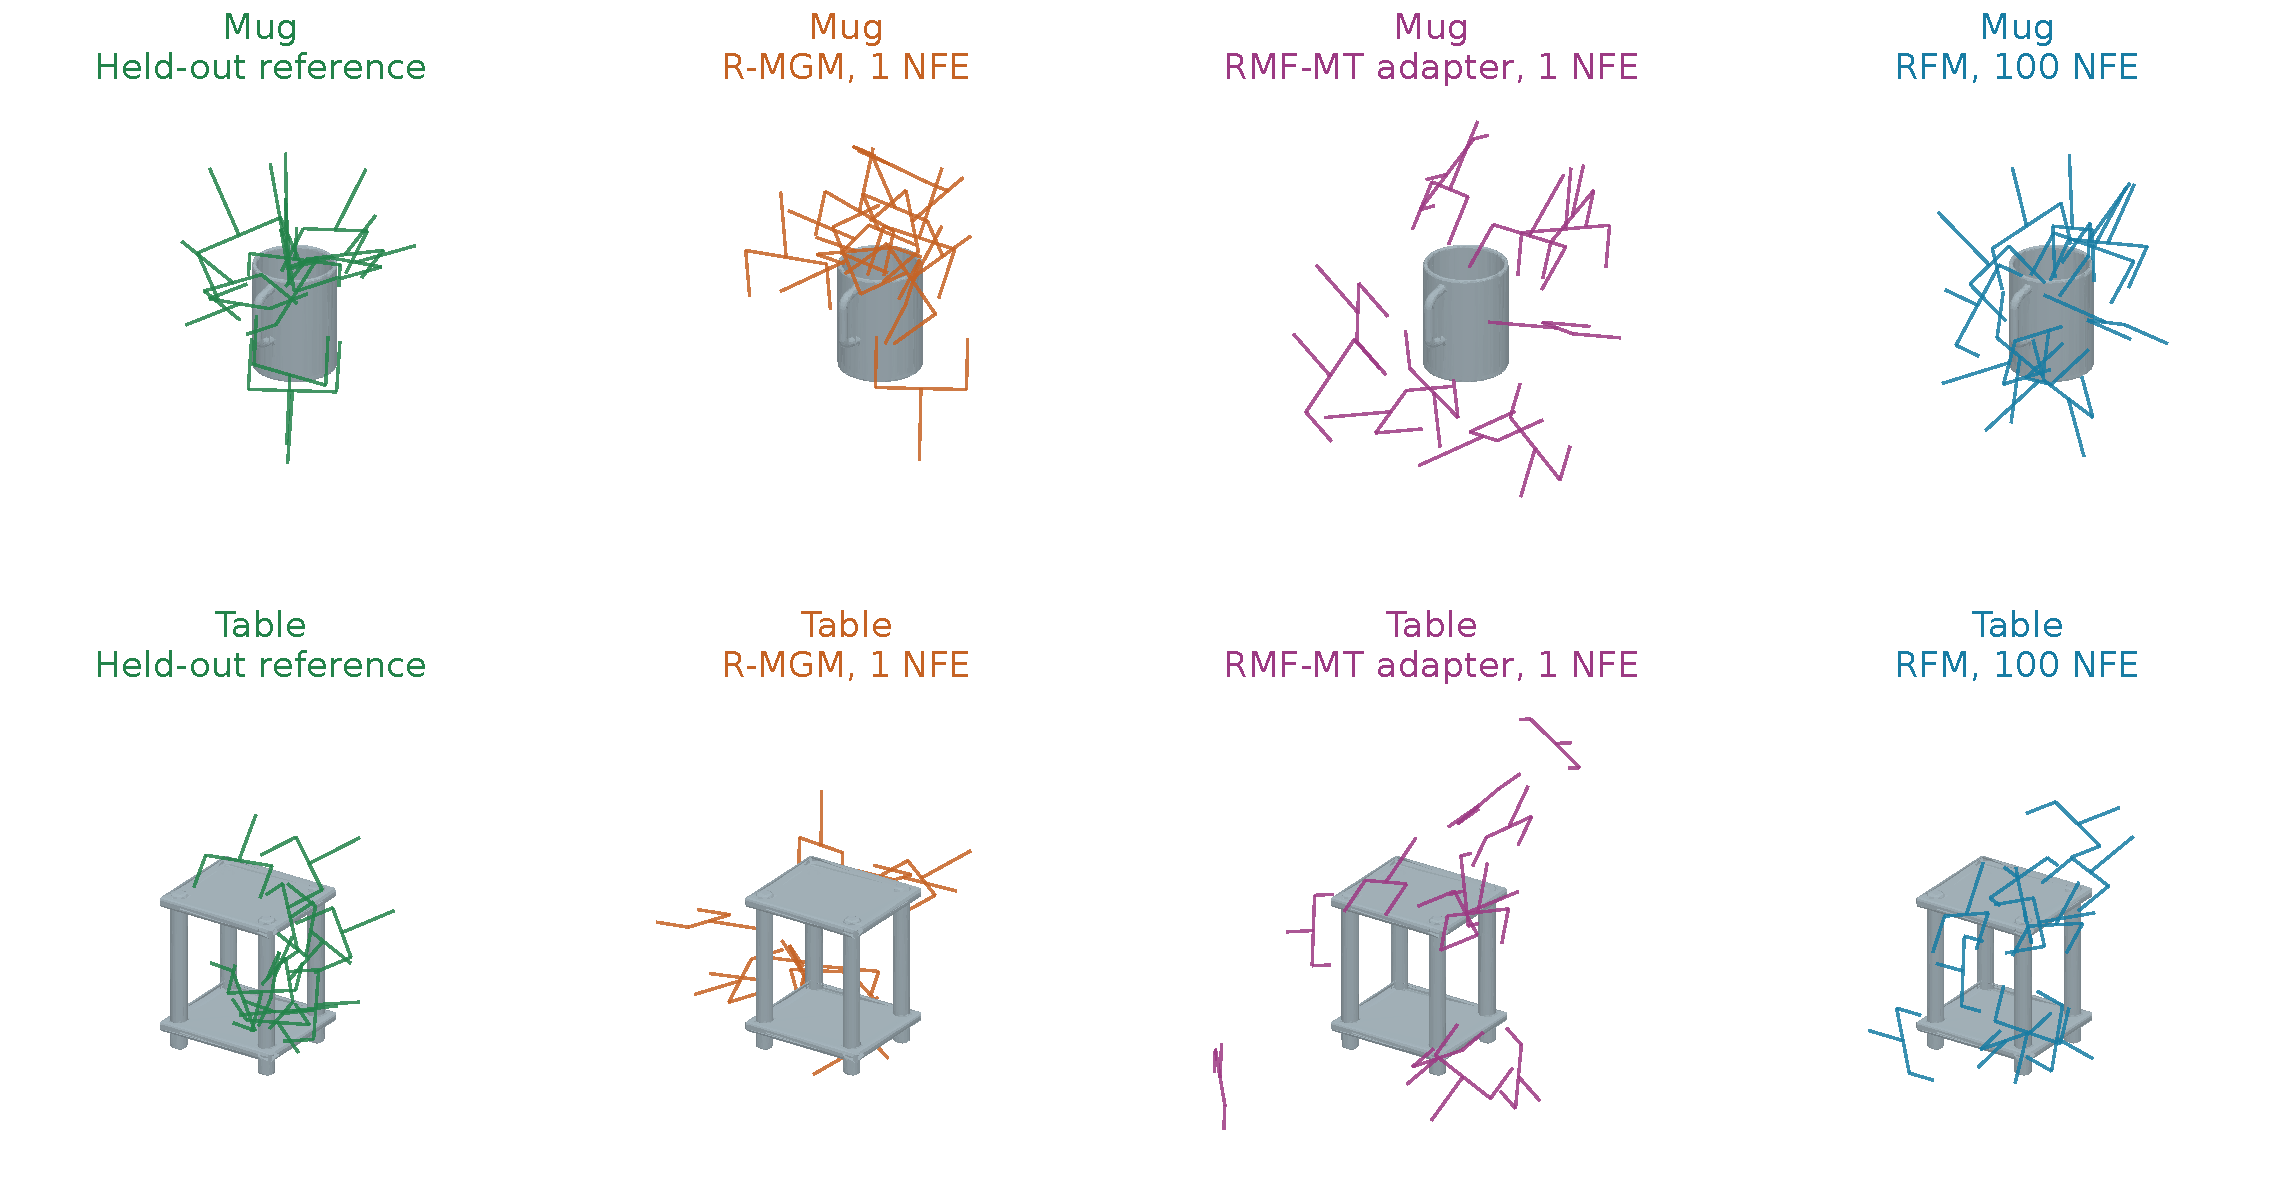
\includegraphics[width=\textwidth]{figures/grasp_current.pdf}
\caption{\textbf{Completed SE(3) pilot on both public objects.} Fixed training seed 0, first 12 unfiltered test draws per method, and a shared camera and metric bounds within each object row. Thin open-gripper centerlines show poses, not physical successes. The common zoom includes every displayed object/gripper vertex; no feasibility filtering or pose replacement is used. This displayed subset is not an all-512-draw tail view. Results aggregate all three training seeds in \cref{tab:grasp}.}
\label{fig:grasp-current}
\end{figure}
\Cref{tab:grasp-object} separates the two known-object test results.
\begin{table}[H]
\centering\small
\caption{Per-object test results over three training seeds. MMD is multiplied by $10^3$; static-proxy and full-collision fractions are percentages. Metrics use 512 generated poses and 100 unfiltered geometry checks per object. These are held-out poses for two known objects, not unseen-object results.}
\label{tab:grasp-object}
\begin{tabular}{@{}lllrrr@{}}
\toprule
Object & Method & NFE & Pose MMD$^2\times10^3$ & Static proxy (\%) & Full collision (\%) \\
\midrule
Mug & R-MGM (ours) & 1 & $5.229\,\pm\,2.052$ & $30.000\,\pm\,2.000$ & $65.667\,\pm\,5.859$ \\
Table & R-MGM (ours) & 1 & $3.301\,\pm\,1.134$ & $19.333\,\pm\,2.887$ & $76.333\,\pm\,7.506$ \\
Mug & RMF-MT adaptation & 1 & $15.207\,\pm\,3.691$ & $17.333\,\pm\,3.786$ & $34.333\,\pm\,4.163$ \\
Table & RMF-MT adaptation & 1 & $8.986\,\pm\,1.064$ & $4.333\,\pm\,1.155$ & $34.000\,\pm\,3.606$ \\
Mug & RFM & 50 & $0.346\,\pm\,0.467$ & $44.000\,\pm\,6.245$ & $66.000\,\pm\,5.568$ \\
Table & RFM & 50 & $0.715\,\pm\,0.487$ & $20.333\,\pm\,1.528$ & $68.000\,\pm\,4.583$ \\
Mug & RFM & 100 & $0.442\,\pm\,0.500$ & $43.667\,\pm\,6.110$ & $65.667\,\pm\,5.508$ \\
Table & RFM & 100 & $0.588\,\pm\,0.504$ & $20.333\,\pm\,0.577$ & $67.667\,\pm\,5.033$ \\
\bottomrule
\end{tabular}
\end{table}

\clearpage
\begin{figure}[H]
\centering
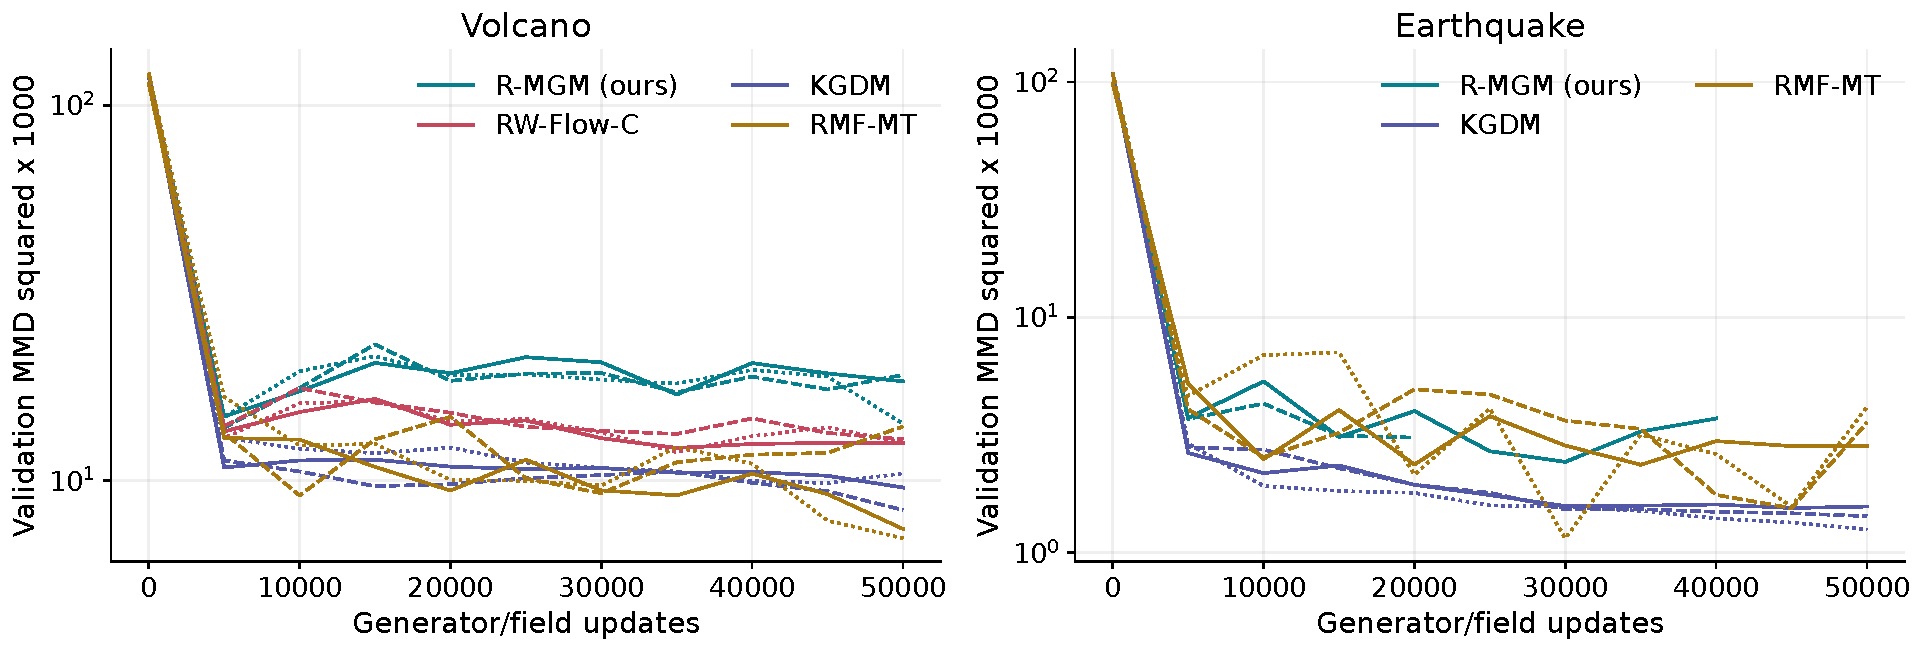
\includegraphics[width=\textwidth]{figures/recent_validation.pdf}
\caption{\textbf{Recorded validation curves at the pause.} Solid, dashed, and dotted lines denote training seeds 0, 1, 2. Earthquake MGM stops at its saved 40,000/20,000-update checkpoints and has no test results. Checkpoint selection includes initialization. These curves are not test scores and do not certify convergence.}
\label{fig:recent-curves}
\end{figure}
\Cref{tab:recent-extra} reports complementary completed-test metrics.
\begin{table}[H]
\centering\small
\caption{Additional completed-test metrics. NN is intrinsic symmetric nearest-neighbor distance in radians (lower is better); coverage uses the fixed training-reference radius (higher is better); 1-NNA has an ideal reference near 0.5. Norm error is mean absolute sphere-unit-norm error. Different metrics need not induce the same ranking.}
\label{tab:recent-extra}
\begin{tabular}{@{}llrrrr@{}}
\toprule
Data & Method & NN & Coverage (\%) & 1-NNA & Norm error \\
\midrule
Volcano & R-MGM (ours) & $0.175\,\pm\,0.021$ & $0.81\,\pm\,0.70$ & $0.728\,\pm\,0.029$ & $3.16e-08$ \\
Volcano & RW-Flow-C & $0.141\,\pm\,0.006$ & $1.90\,\pm\,0.47$ & $0.725\,\pm\,0.010$ & $3.24e-08$ \\
Volcano & KGDM & $0.111\,\pm\,0.008$ & $3.39\,\pm\,0.85$ & $0.674\,\pm\,0.012$ & $3.23e-08$ \\
Volcano & RMF-MT & $0.153\,\pm\,0.014$ & $1.49\,\pm\,1.92$ & $0.762\,\pm\,0.014$ & $3.28e-08$ \\
Earthquake & KGDM & $0.049\,\pm\,0.001$ & $15.43\,\pm\,1.77$ & $0.686\,\pm\,0.005$ & $3.23e-08$ \\
Earthquake & RMF-MT & $0.072\,\pm\,0.004$ & $9.48\,\pm\,2.41$ & $0.769\,\pm\,0.015$ & $3.18e-08$ \\
\bottomrule
\end{tabular}
\end{table}

\clearpage
\section{Earlier Controlled Experimental Protocol}
\label{app:protocol}
\subsection{Fixed Primary Protocol}
Model seeds are 0, 1, 2 and the fixed data-split seed is 0. MLPs have two hidden layers of width 128 (three affine layers), SiLU activations, and a 16-dimensional standard-normal latent. Critics and flow fields use eight Fourier time frequencies and raw wrapped spatial angles on tori. The kernel embedding used for evaluation is a separate circular embedding; it is not the critic input.
All runs use batch 256, float32, AdamW learning rate $2\times10^{-4}$ and weight decay zero. There is one critic update and one generator update per midpoint iteration. No neural-flow teacher is used. The mixture initialization is a train-fitted statistical starting model, not a pretrained flow. Torus mixtures use 64 components for General and 32 for other torsion datasets; sphere mixtures use 12 for Volcano and 24 otherwise. K-means initialization uses at most 8,192 training samples. Hard component selection leaves mixture-weight logits fixed during pathwise training; only centers and scales receive gradients.
The MMD control has the same constrained MLP output map and architecture as the MLP midpoint model and optimizes the biased batch MMD with the fixed training-reference kernel. It is an objective control, not an implementation of a kernel drifting algorithm. Every primary model is evaluated at prespecified steps; validation and test metrics are both saved but neither selects checkpoints or settings. Earlier test exposure is disclosed, so new metrics describe a locked evaluation on an already explored benchmark.
\subsection{Data Counts and Evaluation Size}
Table~\ref{tab:counts} records the local data counts and fixed evaluation size.
\begin{table}[t]\caption{Local preprocessing counts and fixed split sizes. The RNA count is 9,473; it is not asserted to equal every published preprocessing release.}\label{tab:counts}\centering\small\begin{tabular}{@{}lrrrrr@{}}\toprule
Data & Total & Train & Validation & Test & Evaluated $n$ \\
\midrule
Volcano & 827 & 663 & 82 & 82 & 82 \\
Earthquake & 6120 & 4896 & 612 & 612 & 612 \\
Flood & 4875 & 3901 & 487 & 487 & 487 \\
Fire & 12809 & 10249 & 1280 & 1280 & 1024 \\
General & 138208 & 110568 & 13820 & 13820 & 1024 \\
Glycine & 13283 & 10627 & 1328 & 1328 & 1024 \\
Proline & 7634 & 6108 & 763 & 763 & 763 \\
Pre-Pro & 6910 & 5528 & 691 & 691 & 691 \\
RNA (7D) & 9473 & 7579 & 947 & 947 & 947 \\
\bottomrule\end{tabular}\end{table}
All splits are by row. Molecular-source identifiers are not used for group splitting, and geographical rows can be dependent or duplicated. The conclusions concern the specified density-learning protocol, not unseen proteins, independent events, or temporal forecasting.
\subsection{Metrics}
For matched-size samples $x_{1:n}$ and $y_{1:n}$, the reported statistic is
\begin{equation}\widehat{\mathrm{MMD}}_V^2=\frac{1}{n^2}\sum_{i,j=1}^n\big[k(x_i,x_j)+k(y_i,y_j)-2k(x_i,y_j)\big].\end{equation}
The kernel denominator $h^2$ is the median strictly positive squared embedded distance among a fixed random training reference of at most 1,024 points. It is not fitted to generated or test samples. The diagonal terms are included, making this a biased V-statistic with a finite-sample floor; it is not an unbiased estimate. Test and validation targets are sampled without replacement using fixed independent target-selection seeds and reused across models and training seeds.
Nearest-neighbor distances use spherical angles and wrapped Euclidean angle distance on a flat torus. Spherical vectors are normalized in float64 and their angle is computed as $2\operatorname{atan2}(\|\hat x-\hat y\|_2,\|\hat x+\hat y\|_2)$, avoiding false positive distances between identical float32 directions. Symmetric NN is one half the sum of the two directed mean nearest distances. Coverage is the fraction of fixed target points within radius $r$ of a generated point; $r$ is the median positive leave-one-out nearest distance on the fixed training reference. Identical normalized directions are explicitly excluded from the sphere reference calibration. Mesh distances below are ambient Euclidean, not intrinsic geodesic distances.
Three generated draws are averaged within each training seed, followed by mean and sample standard deviation across the three independent training seeds. Draws are Monte Carlo replicates, not extra training seeds. Sphere validity is mean absolute unit-norm error. Torus validity is the fraction outside the half-open angle interval $[0,2\pi)$.
\subsection{Sampling and Compute}
The controlled RFM uses projected/exponential Euler with midpoint-in-time evaluation and one actual vector-field call per step. Both 1- and 128-NFE cases are saved at each prespecified checkpoint. Forward hooks verify counts. CUDA is synchronized around timing; GPU warmups and metric calculations are excluded. Single-thread CPU timing uses three repeated batches. Data preparation and mixture initialization are separately recorded, and training duration excludes evaluation pauses. This is not a claim of identical training FLOPs or total wall-clock cost across algorithms.
The final controlled bundle contains 72 completed training jobs, with 17.03 minutes of summed synchronized training time. This sum excludes evaluation, setup, discarded preliminary reruns, exploratory historical jobs, and incomplete attempts; it is not total project GPU time. Hardware: one NVIDIA GeForce RTX 4090, PyTorch 2.5.1 with CUDA 12.1. Other GPU processes were observed during part of this bundle; synchronized durations are actual wall times, not isolated hardware costs or proof of a speedup. Individual runs record their own durations.
\subsection{Randomness and Metric Audit}
A timing-helper audit exposed evaluation-induced resetting of a global CUDA stream in the preliminary GMM/RFM runs. The final bundle replaces all 54 affected runs using frozen sources and separate target, latent, time/flip, and flow-base RNG streams derived from model seed. It copies the 18 unaffected MLP objective-control jobs with file hashes. Evaluation is asserted to preserve all training streams at every checkpoint. Rerun checkpoints save optimizer and CPU/CUDA/private RNG states; the copied earlier MLP checkpoints are suitable for reevaluation but lack full continuation state. GPU reductions are not guaranteed bitwise identical across devices.
A separate analysis-only correction recomputes sphere angles and coverage from saved arrays with the normalized float64 metric above. Raw metric JSONs are archived with correction hashes, and training sources and generated arrays are unchanged. The final-table marker requires the corrected metric version. Both audits precede the final aggregation; neither selects models by their test scores.
\subsection{Reproduction Commands}
From the repository root with the provided conda environment, the following commands check and render the final recorded bundle. The experiment README gives the ordered training, immutable-snapshot rerun, metric-correction, and validation-only commands for a clean reconstruction.
\begingroup\small\begin{verbatim}
python paper/experiments/verify_independent.py
python paper/check_geometry.py
python paper/make_illustrations.py
python paper/update_results.py --run-root controlled_independent --require-complete
powershell -File paper/build.ps1
\end{verbatim}\endgroup
Data/split hashes and executed-code hashes accompany the final result ledger. Natural Earth public-domain land outlines are used only as geographic context in maps; density color fields are computed from saved samples.
Display KDEs are separate from the evaluation MMD kernel. Spherical plots use a normalized von Mises--Fisher kernel with concentration 45 (density per steradian); torus plots smooth a 120-by-120 periodic histogram using Gaussian sigma 2.4 bins and divide by angular bin area (density per squared radian). Comparisons use one logarithmic color scale and clip values below $10^{-3}$ of the maximum within that comparison. Horizontal geographic and angle domains span $[-180,180]$ degrees; only the first two RNA angles are displayed.

\section{Validation-Only Optimization Diagnostics}
\label{app:stability}
This post hoc diagnostic was motivated by the primary failures. It uses General training data and its fixed validation target only, model seed 0, and three generated draws per probe. No new test score is obtained or used to choose a candidate. Trials are reported together rather than replacing the unsuccessful primary setting. These exploratory results do not establish cross-seed robustness.
Table~\ref{tab:stability} records the initial and final validation outcomes.
\begin{table}[t]\caption{Validation-only General optimization study. All values are means of three Monte Carlo draws from one seed-0 model, not independent training replicates. MMD columns are multiplied by $10^3$; optimizer counts include critic warmup.}\label{tab:stability}\centering\small
\begin{tabular}{@{}llrrrrr@{}}\toprule
Configuration & Generator LR & Gen./field steps & Total updates & Initial val. & Final val. & Train s \\
\midrule
Raw random MLP, C=5 & 1e-05 & 2000 & 12500 & 750.34 & 256.37 & 19.8 \\
Periodic random MLP, C=5 & 1e-05 & 2000 & 12500 & 750.34 & 292.37 & 20.6 \\
Periodic random GMM, C=5 & 1e-05 & 2000 & 12500 & 203.86 & 199.85 & 20.8 \\
Periodic train-fit GMM, C=5 & 1e-05 & 2000 & 12500 & 0.82 & 0.83 & 20.7 \\
Periodic random MLP, C=10 & 1e-05 & 2000 & 22500 & 750.34 & 298.39 & 34.9 \\
Periodic RFM & 2e-04 & 22500 & 22500 & 195.40 & 1.91 & 30.4 \\
Periodic random MLP, C=5 & 2e-04 & 10000 & 60500 & 750.34 & 34.91 & 164.3 \\
Periodic random GMM, C=5 & 2e-04 & 10000 & 60500 & 203.86 & 16.40 & 171.0 \\
Periodic random MLP, C=5 & 1e-04 & 2000 & 12500 & 750.34 & 40.23 & 20.7 \\
Periodic random MLP, C=5 & 2e-04 & 2000 & 12500 & 750.34 & 35.00 & 20.8 \\
\bottomrule\end{tabular}\end{table}
The periodic critic/field uses sine and cosine spatial harmonics 1--4, eight Fourier time frequencies, width 128, and three affine layers. The study adds 500 critic-only warmup updates, five or ten critic updates per generator iteration, and slower generator learning rates, with the higher-rate refinement recorded separately. Its flow control uses the same periodic field architecture and fixed update counts; it must not be confused with the raw-angle controlled RFM in the primary table.
Figure~\ref{fig:stability} shows illustrative configurations from this post hoc study.
\begin{figure}[t]\centering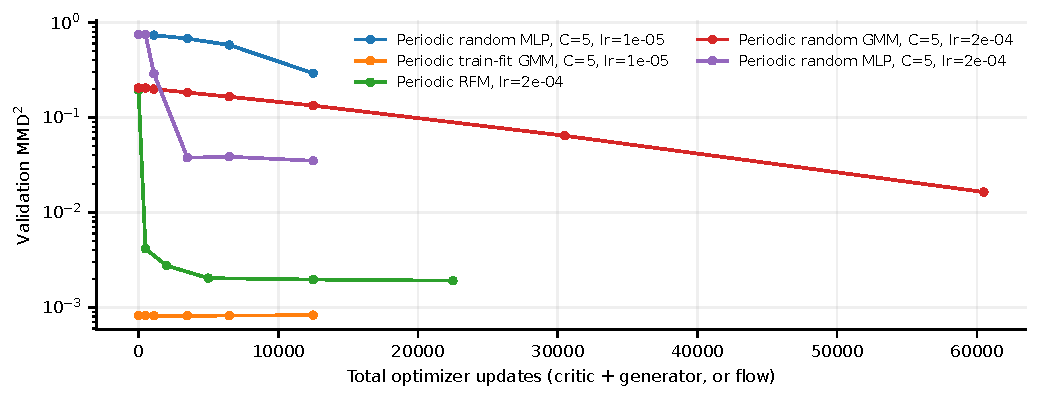
\includegraphics[width=\textwidth]{figures/validation_stability.pdf}
\caption{General validation diagnostics from one training seed. Lines join fixed probe checkpoints; they are not interpolated test estimates. Curves illustrate retention, random initialization, higher-rate refinement, and periodic RFM; all completed trial outcomes are listed in Table~\ref{tab:stability}. Update counts are not equal FLOPs; measured training times appear in the table.}\label{fig:stability}\end{figure}

\subsection{True-Velocity Randomized Paths}
We separately probe the reversible randomized torus path in \cref{eq:noisy-torus} on General, with $\varepsilon\in\{0,0.3,0.7\}$. The actual derivative includes the noise-amplitude derivative. The experiment uses a randomly initialized MLP, the periodic critic, seed 0, batch 512, 10,000 generator updates, five critic updates per generator step, 500 critic warmup updates, and generator/critic learning rates $2\times10^{-4}$. All three amplitudes and fixed checkpoints are specified before this diagnostic. It is post hoc validation-only evidence, not a replacement for the primary table or independent-seed confirmation. Evaluation preserves the training RNG state.
Table~\ref{tab:noise} lists every amplitude. Figure~\ref{fig:noise} shows the fixed-checkpoint validation curves. The $\varepsilon=0$ row is a separately executed deterministic control with the same code path and random draws, not a copied earlier result.
\begin{table}[t]\caption{Randomized-torus validation diagnostic. One seed-0 model per amplitude; MMD$^2\times10^3$ means average three sampling draws. The final SD is Monte Carlo variation only. No test metrics are evaluated.}\label{tab:noise}\centering\small\begin{tabular}{@{}rrrrr@{}}\toprule
Amplitude $\varepsilon$ & Initial val. & Final val. & Final MC SD & Train s \\
\midrule
0 & 750.34 & 60.70 & 3.86 & 159.9 \\
0.3 & 750.34 & 36.53 & 1.85 & 156.0 \\
0.7 & 750.34 & 31.68 & 0.71 & 150.2 \\
\bottomrule\end{tabular}\end{table}
Noise improves the final validation MMD relative to this deterministic control in the single-seed sweep, but all three models remain above the periodic RFM reference (approximately $1.91\times10^{-3}$). Their 60,500 total optimizer updates exceed that reference's 22,500 field updates; neither update counts nor FLOPs are matched. This diagnostic does not establish cross-seed efficacy or an advantage over the flow.
\begin{figure}[t]\centering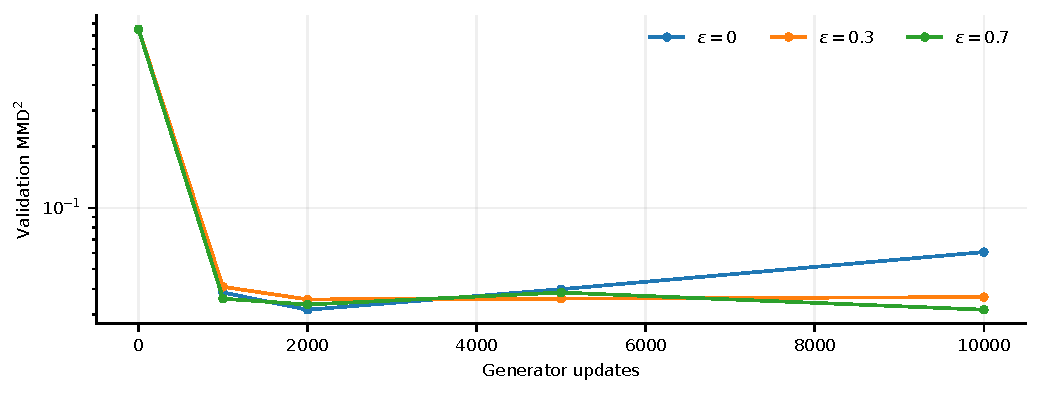
\includegraphics[width=\textwidth]{figures/validation_noise.pdf}
\caption{Validation-only true-velocity noise diagnostic. Lines join prespecified checkpoints for three seed-0 models. Different amplitudes define different path discrepancies; these curves do not estimate the population divergence or establish a generally optimal noise level.}\label{fig:noise}\end{figure}

\clearpage
\section{Additional Quantitative and Qualitative Results}
\label{app:additional}
\begin{figure}[t]
\centering
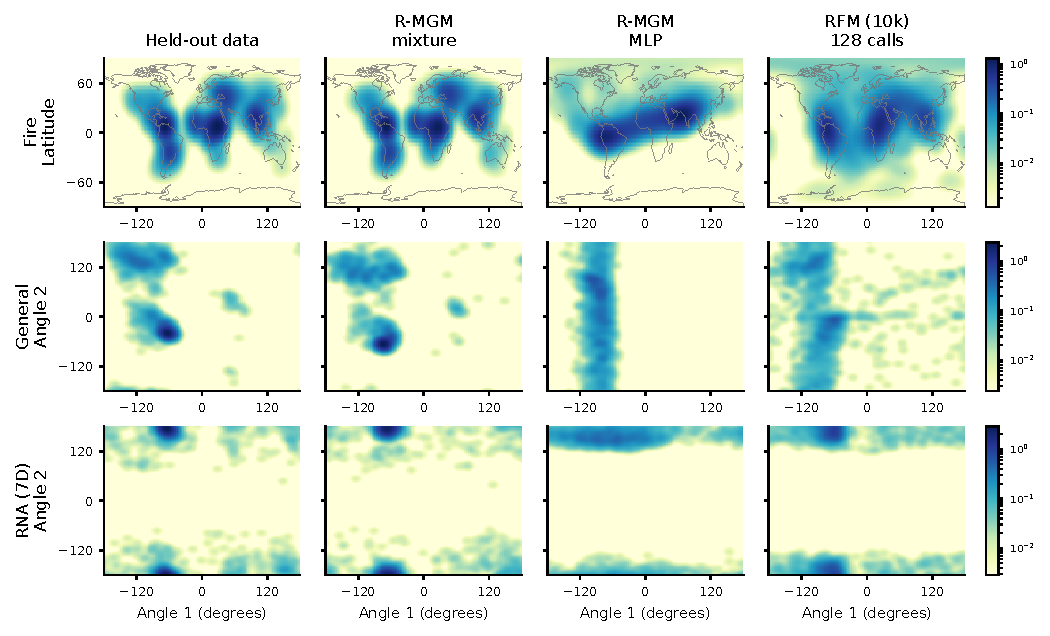
\includegraphics[width=\textwidth]{figures/controlled_samples.pdf}
\caption{\textbf{Earlier controlled study.} Fixed test target and training seed 0. Fire uses spherical KDE; General and the first two RNA angles use periodic KDE. These earlier mixture/flow models are distinct from the unfitted-generator modern protocol. Each row uses the same logarithmic color scale. These are sample densities, not model likelihoods or full-joint RNA validation.}
\label{fig:controlled}
\end{figure}
\begin{table}[t]
\caption{\textbf{Sampling latency on Fire.} Milliseconds per batch of 1,024, mean $\pm$ SD over training-seed means; CUDA-synchronized GPU and single-thread CPU measurements exclude warmup. Calls count a generator or a field evaluation; the mixture map is not a neural network. RNG and constraints are included.}
\label{tab:latency}
\centering\small
\begin{tabular}{@{}lrrr@{}}
\toprule
Method & Calls & GPU ms & CPU ms \\
\midrule
R-MGM GMM & 1 & $2.12\,\pm\,2.54$ & $0.31\,\pm\,0.00$ \\
R-MGM MLP & 1 & $0.80\,\pm\,0.04$ & $0.83\,\pm\,0.03$ \\
MMD MLP & 1 & $0.47\,\pm\,0.05$ & $0.57\,\pm\,0.01$ \\
RFM (1) & 1 & $2.10\,\pm\,0.69$ & $0.87\,\pm\,0.04$ \\
RFM (128) & 128 & $37.83\,\pm\,1.51$ & $83.92\,\pm\,0.42$ \\
\bottomrule
\end{tabular}
\end{table}

\begin{figure}[t]
\centering
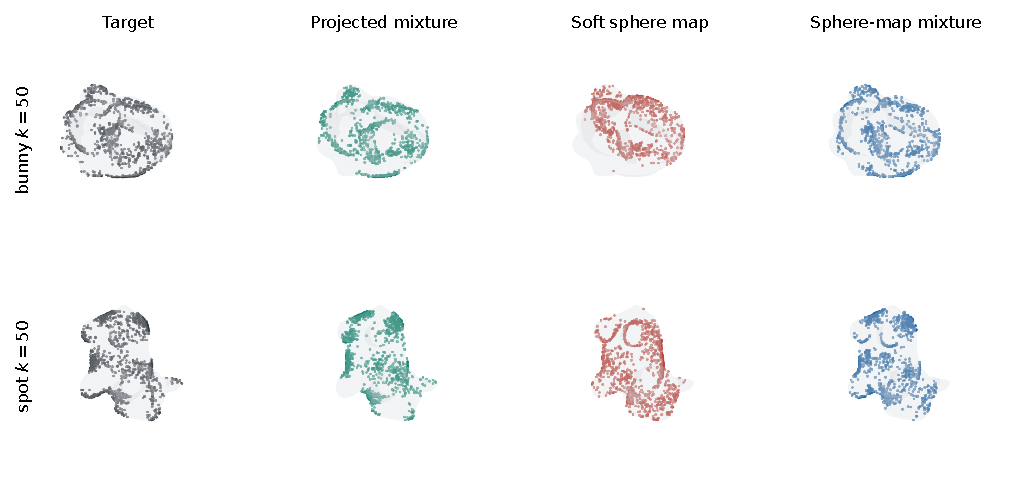
\includegraphics[width=\textwidth]{figures/mesh_selected.pdf}
\caption{\textbf{Exploratory surface generation.} Fixed final checkpoints on Bunny $k=50$ and Spot $k=50$, with identical cameras and 1,024 points in each panel. Columns show target samples and three constrained-generator variants. All use the local projected-chord surrogate; the soft sphere map is not a certified bijection. Qualitative resemblance and output validity do not establish agreement of intrinsic densities.}
\label{fig:mesh}
\end{figure}
\subsection{Full Sample Metrics}
Table~\ref{tab:all-metrics} supplements Table~\ref{tab:main} with distances, coverage, and validity.
\begin{table}[t]\caption{Additional controlled test metrics, mean $\pm$ training-seed SD for NN and coverage. Validity reports the mean error defined in the text.}\label{tab:all-metrics}\centering\small\begin{tabular}{@{}llrrr@{}}\toprule
Data & Method / updates & Symmetric NN $\downarrow$ & Coverage $\uparrow$ & Validity error $\downarrow$ \\
\midrule
Volcano & R-MGM mixture / 2k & $0.119\,\pm\,0.021$ & $0.028\,\pm\,0.019$ & $3.0e-08$ \\
Volcano & RFM / 2k & $0.204\,\pm\,0.003$ & $0.005\,\pm\,0.006$ & $3.3e-08$ \\
Volcano & RFM / 10k & $0.189\,\pm\,0.003$ & $0.005\,\pm\,0.005$ & $3.5e-08$ \\
Earthquake & R-MGM mixture / 2k & $0.044\,\pm\,0.001$ & $0.156\,\pm\,0.006$ & $3.2e-08$ \\
Earthquake & RFM / 2k & $0.101\,\pm\,0.000$ & $0.054\,\pm\,0.003$ & $3.5e-08$ \\
Earthquake & RFM / 10k & $0.079\,\pm\,0.001$ & $0.092\,\pm\,0.009$ & $3.5e-08$ \\
Flood & R-MGM mixture / 2k & $0.052\,\pm\,0.001$ & $0.123\,\pm\,0.022$ & $3.0e-08$ \\
Flood & RFM / 2k & $0.097\,\pm\,0.001$ & $0.062\,\pm\,0.004$ & $3.4e-08$ \\
Flood & RFM / 10k & $0.087\,\pm\,0.001$ & $0.073\,\pm\,0.012$ & $3.4e-08$ \\
Fire & R-MGM mixture / 2k & $0.028\,\pm\,0.002$ & $0.144\,\pm\,0.015$ & $3.0e-08$ \\
Fire & RFM / 2k & $0.087\,\pm\,0.001$ & $0.022\,\pm\,0.000$ & $3.5e-08$ \\
Fire & RFM / 10k & $0.067\,\pm\,0.002$ & $0.035\,\pm\,0.001$ & $3.4e-08$ \\
General & R-MGM mixture / 2k & $0.096\,\pm\,0.019$ & $0.198\,\pm\,0.092$ & $0.0e+00$ \\
General & RFM / 2k & $0.166\,\pm\,0.001$ & $0.203\,\pm\,0.010$ & $0.0e+00$ \\
General & RFM / 10k & $0.132\,\pm\,0.001$ & $0.269\,\pm\,0.006$ & $0.0e+00$ \\
Glycine & R-MGM mixture / 2k & $0.172\,\pm\,0.033$ & $0.091\,\pm\,0.043$ & $0.0e+00$ \\
Glycine & RFM / 2k & $0.161\,\pm\,0.002$ & $0.118\,\pm\,0.004$ & $0.0e+00$ \\
Glycine & RFM / 10k & $0.114\,\pm\,0.003$ & $0.238\,\pm\,0.006$ & $0.0e+00$ \\
Proline & R-MGM mixture / 2k & $0.136\,\pm\,0.011$ & $0.064\,\pm\,0.029$ & $0.0e+00$ \\
Proline & RFM / 2k & $0.230\,\pm\,0.002$ & $0.104\,\pm\,0.012$ & $0.0e+00$ \\
Proline & RFM / 10k & $0.101\,\pm\,0.007$ & $0.213\,\pm\,0.014$ & $0.0e+00$ \\
Pre-Pro & R-MGM mixture / 2k & $0.061\,\pm\,0.016$ & $0.316\,\pm\,0.062$ & $0.0e+00$ \\
Pre-Pro & RFM / 2k & $0.157\,\pm\,0.002$ & $0.204\,\pm\,0.006$ & $0.0e+00$ \\
Pre-Pro & RFM / 10k & $0.134\,\pm\,0.004$ & $0.246\,\pm\,0.026$ & $0.0e+00$ \\
RNA (7D) & R-MGM mixture / 2k & $0.396\,\pm\,0.002$ & $0.314\,\pm\,0.010$ & $0.0e+00$ \\
RNA (7D) & RFM / 2k & $0.965\,\pm\,0.004$ & $0.000\,\pm\,0.000$ & $0.0e+00$ \\
RNA (7D) & RFM / 10k & $0.736\,\pm\,0.013$ & $0.041\,\pm\,0.015$ & $0.0e+00$ \\
\bottomrule\end{tabular}\end{table}
Spherical NN units are radians. Torus NN uses the Euclidean norm of wrapped angular differences in radians. The coverage threshold is fixed separately per dataset from training data. Validity means unit-norm error on a sphere and out-of-range fraction on a torus; these different quantities must not be averaged across domains.
\subsection{Matched MLP Objective Controls}
Figure~\ref{fig:objective-controls} visualizes the parameterization-matched models from training seed 0.
\begin{figure}[t]\centering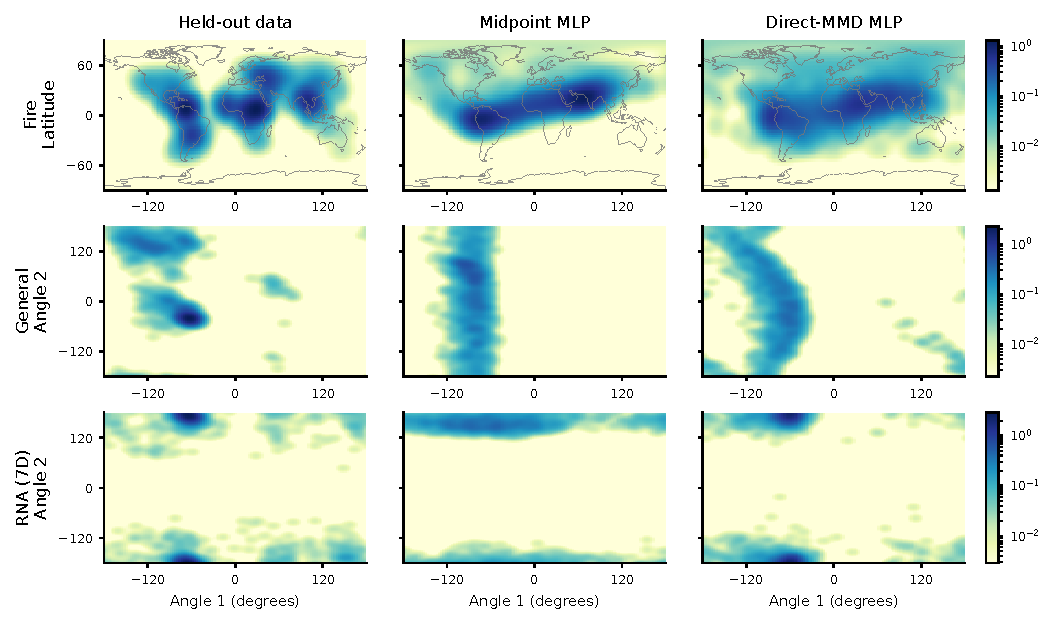
\includegraphics[width=\textwidth]{figures/objective_controls.pdf}
\caption{Matched constrained MLPs after 2,000 updates: the same fixed test targets and training seed 0, with midpoint and direct-MMD objectives. Each row uses one logarithmic KDE scale and the plotting convention of Figure~\ref{fig:controlled}. Only the first two RNA angles are displayed. These are sample densities, not model likelihoods.}\label{fig:objective-controls}\end{figure}
Table~\ref{tab:mlp-metrics} supplements the matched-architecture objective comparison with non-MMD metrics. The MMD control directly optimizes the evaluation kernel, so its MMD advantage alone would not establish superiority on all distributional criteria.
\begin{table}[t]\caption{Matched MLP controls at 2,000 generator updates. Mean and sample SD across three training seeds, after averaging three draws per seed. Smaller symmetric NN and larger coverage are better.}\label{tab:mlp-metrics}\centering\small\begin{tabular}{@{}llrr@{}}\toprule
Data & Objective & Symmetric NN & Coverage \\
\midrule
Fire & Midpoint & $0.115\,\pm\,0.011$ & $0.024\,\pm\,0.017$ \\
Fire & Direct MMD & $0.080\,\pm\,0.002$ & $0.030\,\pm\,0.004$ \\
General & Midpoint & $0.168\,\pm\,0.022$ & $0.196\,\pm\,0.026$ \\
General & Direct MMD & $0.158\,\pm\,0.004$ & $0.257\,\pm\,0.011$ \\
RNA (7D) & Midpoint & $0.913\,\pm\,0.225$ & $0.000\,\pm\,0.000$ \\
RNA (7D) & Direct MMD & $0.508\,\pm\,0.016$ & $0.111\,\pm\,0.039$ \\
\bottomrule\end{tabular}\end{table}
\subsection{Numerical Geometry Audits}
Table~\ref{tab:geometry-audit} reports the interpolation residuals.
\begin{table}[t]\caption{Maximum numerical residuals over 64 float64 endpoint pairs per geometry. Position and derivative-comparison norms are ambient; velocity reversal uses the manifold metric.}\label{tab:geometry-audit}\centering\small\begin{tabular}{@{}lrrr@{}}\toprule
Geometry & Position reversal & Velocity reversal & Velocity vs. finite difference \\
\midrule
sphere & $2.38e-14$ & $3.48e-15$ & $2.88e-10$ \\
torus & $1.28e-15$ & $0.00e+00$ & $5.36e-10$ \\
spd & $1.63e-15$ & $5.96e-16$ & $6.58e-10$ \\
hyperbolic & $7.09e-08$ & $8.02e-08$ & $8.37e-08$ \\
\bottomrule\end{tabular}\end{table}
The hyperbolic target itself is approximate. The audited endpoint distribution is not an exhaustive numerical guarantee.
\subsection{Empirical Training-Resampling Reference}
Table~\ref{tab:resampling} calibrates the sample estimator using direct resampling from the empirical training distribution. It is a memorization reference, not a learned generator or a universal lower bound on MMD.
\begin{table}[t]\caption{Empirical training resampling against the fixed test targets. Mean and Monte Carlo SD over three draws; there are zero training seeds in these reference rows.}\label{tab:resampling}\centering\small\begin{tabular}{@{}lrrr@{}}\toprule
Data & MMD$^2\times10^3$ & Symmetric NN & Coverage \\
\midrule
Volcano & $13.390\pm6.585$ & $0.062\pm0.004$ & $0.447\pm0.078$ \\
Earthquake & $1.632\pm0.658$ & $0.024\pm0.001$ & $0.381\pm0.030$ \\
Fire & $0.796\pm0.288$ & $0.012\pm0.001$ & $0.441\pm0.031$ \\
Flood & $1.833\pm1.152$ & $0.034\pm0.002$ & $0.324\pm0.016$ \\
General & $0.992\pm0.732$ & $0.037\pm0.001$ & $0.525\pm0.011$ \\
Glycine & $1.144\pm0.464$ & $0.054\pm0.000$ & $0.476\pm0.009$ \\
Proline & $0.499\pm0.242$ & $0.025\pm0.000$ & $0.421\pm0.007$ \\
Pre-Pro & $1.321\pm0.476$ & $0.040\pm0.002$ & $0.392\pm0.012$ \\
RNA (7D) & $1.871\pm0.649$ & $0.269\pm0.006$ & $0.499\pm0.008$ \\
\bottomrule\end{tabular}\end{table}
\begin{figure}[t]\centering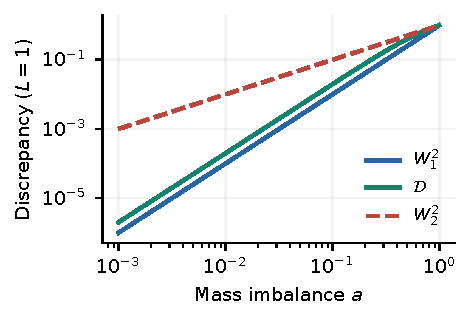
\includegraphics[width=.48\textwidth]{figures/transport_bounds.pdf}
\caption{Exact two-point example from Appendix~\ref{app:proofs}. The midpoint discrepancy controls $W_1^2$ but need not control $W_2^2$ by a universal linear constant. Curves are analytic, not learned-model estimates.}\label{fig:bounds}\end{figure}
\subsection{Historical Additional-Geometry Pilots}
The following historical runs use the legacy metric estimator and one training seed. Its kernel was fitted from generated and target points, and test metrics were monitored during development. We report final steps only, but historical tuning exposure remains. Values are exploratory and must not be pooled with the new fixed-kernel, three-seed tables. Paired-source tasks were adapted to target-only generation by retaining $x_1$; therefore the maze and hyperbolic rows do not reproduce the original source-to-target transport experiment.
Table~\ref{tab:legacy-extra} records all matching historical final-step runs, including repeated configurations rather than selecting the best observed result.
\begin{table}[t]\caption{Historical additional-geometry pilots with their original estimator. Repeated task/method rows are separate configurations; these values are not comparable to the new fixed-kernel table.}\label{tab:legacy-extra}\centering\small\begin{tabular}{@{}llrrrr@{}}\toprule
Task & Method & Dimension & Steps & Legacy MMD$^2$ & Legacy sym. NN \\
\midrule
hyperbolic & Light RFM & 2 & 2000 & 0.0151 & 0.0269 \\
hyperbolic & R-MGM & 2 & 2000 & 0.0108 & 0.0089 \\
maze3v2 & Light RFM & 3 & 500 & 0.1210 & 0.1473 \\
maze3v2 & R-MGM & 3 & 500 & 0.2446 & 0.1293 \\
maze3v2 & R-MGM & 3 & 500 & 0.0009 & 0.0052 \\
maze4v2 & Light RFM & 3 & 500 & 0.0613 & 0.1321 \\
maze4v2 & R-MGM & 3 & 500 & 0.0050 & 0.0078 \\
simple\_bunny & Light RFM & 3 & 500 & 0.5121 & 0.3097 \\
simple\_bunny & R-MGM & 3 & 500 & 0.0023 & 0.0051 \\
wrapped\_spd & Light RFM & 3 & 2000 & 0.0051 & 0.1122 \\
wrapped\_spd & R-MGM & 3 & 2000 & 0.0096 & 0.1144 \\
wrapped\_torus & Light RFM & 5 & 2000 & 0.1912 & 0.5299 \\
wrapped\_torus & R-MGM & 5 & 2000 & 0.0007 & 0.1218 \\
wrapped\_spd & Light RFM & 6 & 1000 & 0.0101 & 0.3962 \\
wrapped\_spd & Light RFM & 10 & 1000 & 0.0067 & 0.7417 \\
wrapped\_spd & R-MGM & 6 & 1000 & 0.0296 & 0.4868 \\
wrapped\_spd & R-MGM & 6 & 1000 & 0.0087 & 0.4137 \\
wrapped\_spd & R-MGM & 10 & 1000 & 0.0169 & 0.8048 \\
wrapped\_torus & Light RFM & 10 & 1000 & 0.4044 & 1.6642 \\
wrapped\_torus & Light RFM & 20 & 1000 & 0.4979 & 3.6284 \\
wrapped\_torus & R-MGM & 10 & 1000 & 0.0010 & 0.3639 \\
wrapped\_torus & R-MGM & 20 & 1000 & 0.0010 & 0.7266 \\
\bottomrule\end{tabular}\end{table}
Wrapped-SPD vector dimensions 3, 6, 10 correspond to matrix sizes 2, 3, 4. They are synthetic data, not EEG covariance models. The high-dimensional torus pilots cover dimensions 5, 10 and 20 only; they are not the full author scaling sweep.
Figure~\ref{fig:extra-volcano} shows the fixed-seed comparison for Volcano.
\begin{figure*}[t]\centering
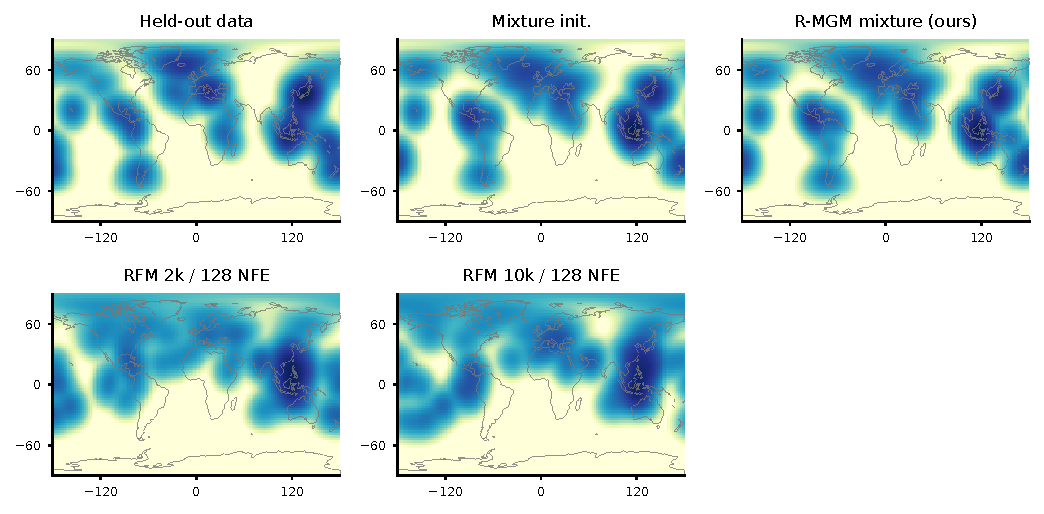
\includegraphics[width=\textwidth]{figures/volcano_comparison.pdf}
\caption{Volcano: fixed test target and training seed 0. Columns are labeled with their generator or flow training budget. Common-bandwidth sample KDEs use the same scale within this figure; these are not likelihood plots.}\label{fig:extra-volcano}\end{figure*}
Figure~\ref{fig:extra-earthquake} shows the fixed-seed comparison for Earthquake.
\begin{figure*}[t]\centering
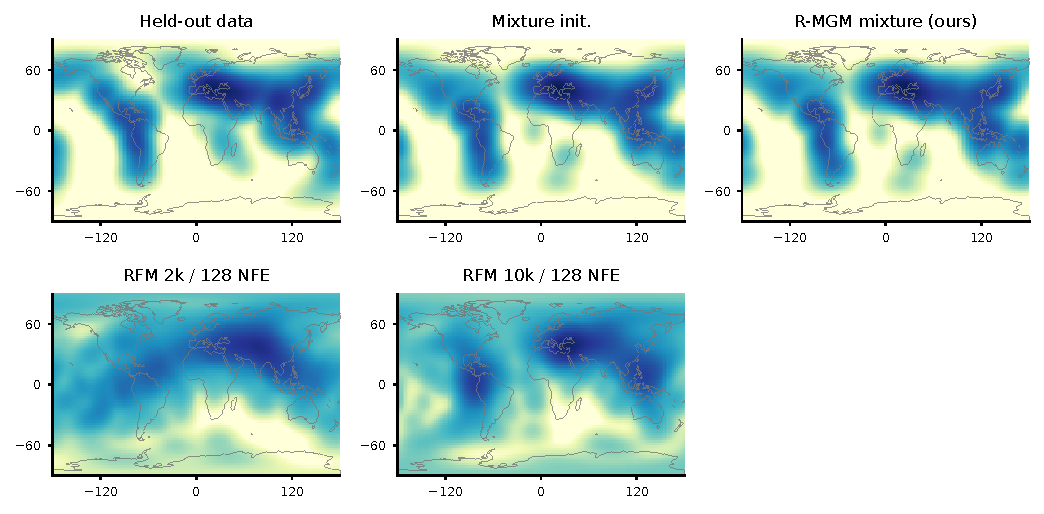
\includegraphics[width=\textwidth]{figures/earthquake_comparison.pdf}
\caption{Earthquake: fixed test target and training seed 0. Columns are labeled with their generator or flow training budget. Common-bandwidth sample KDEs use the same scale within this figure; these are not likelihood plots.}\label{fig:extra-earthquake}\end{figure*}
Figure~\ref{fig:extra-flood} shows the fixed-seed comparison for Flood.
\begin{figure*}[t]\centering
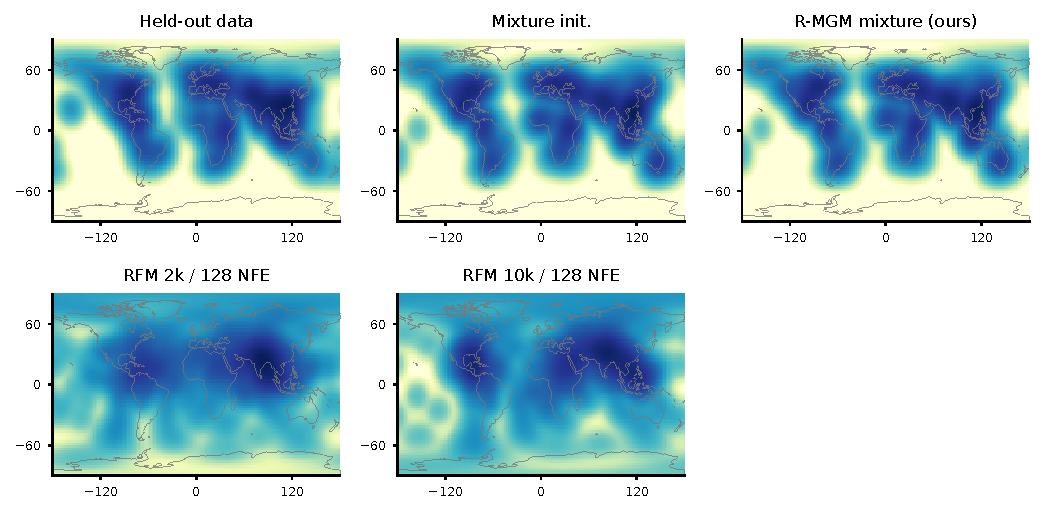
\includegraphics[width=\textwidth]{figures/flood_comparison.pdf}
\caption{Flood: fixed test target and training seed 0. Columns are labeled with their generator or flow training budget. Common-bandwidth sample KDEs use the same scale within this figure; these are not likelihood plots.}\label{fig:extra-flood}\end{figure*}
Figure~\ref{fig:extra-fire} shows the fixed-seed comparison for Fire.
\begin{figure*}[t]\centering
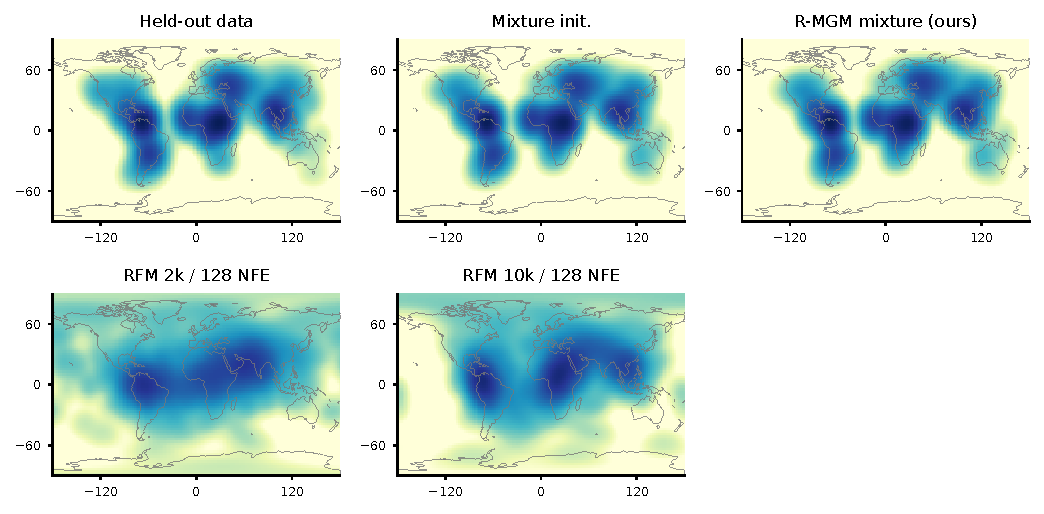
\includegraphics[width=\textwidth]{figures/fire_comparison.pdf}
\caption{Fire: fixed test target and training seed 0. Columns are labeled with their generator or flow training budget. Common-bandwidth sample KDEs use the same scale within this figure; these are not likelihood plots.}\label{fig:extra-fire}\end{figure*}
Figure~\ref{fig:extra-general} shows the fixed-seed comparison for General.
\begin{figure*}[t]\centering
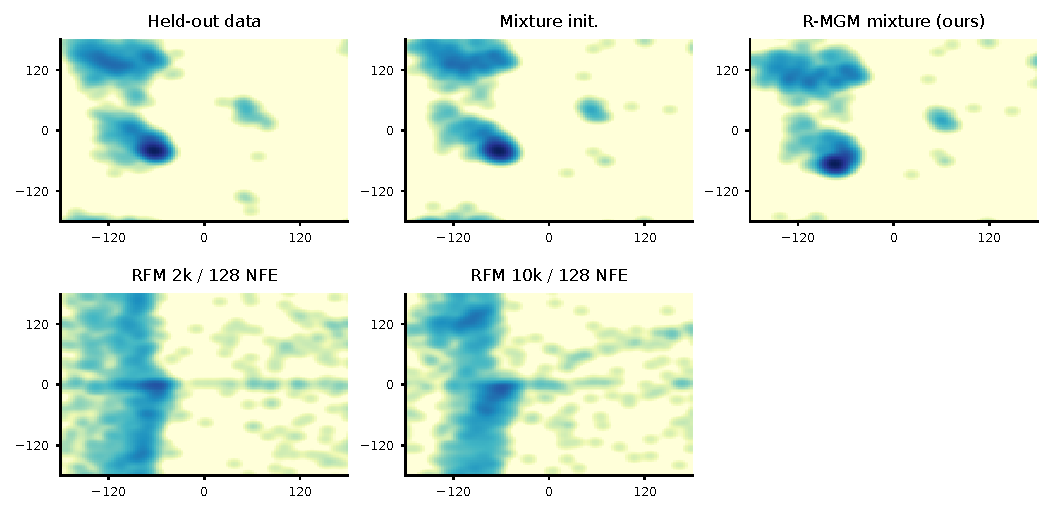
\includegraphics[width=\textwidth]{figures/general_comparison.pdf}
\caption{General: fixed test target and training seed 0. Columns are labeled with their generator or flow training budget. Common-bandwidth sample KDEs use the same scale within this figure; these are not likelihood plots.}\label{fig:extra-general}\end{figure*}
Figure~\ref{fig:extra-glycine} shows the fixed-seed comparison for Glycine.
\begin{figure*}[t]\centering
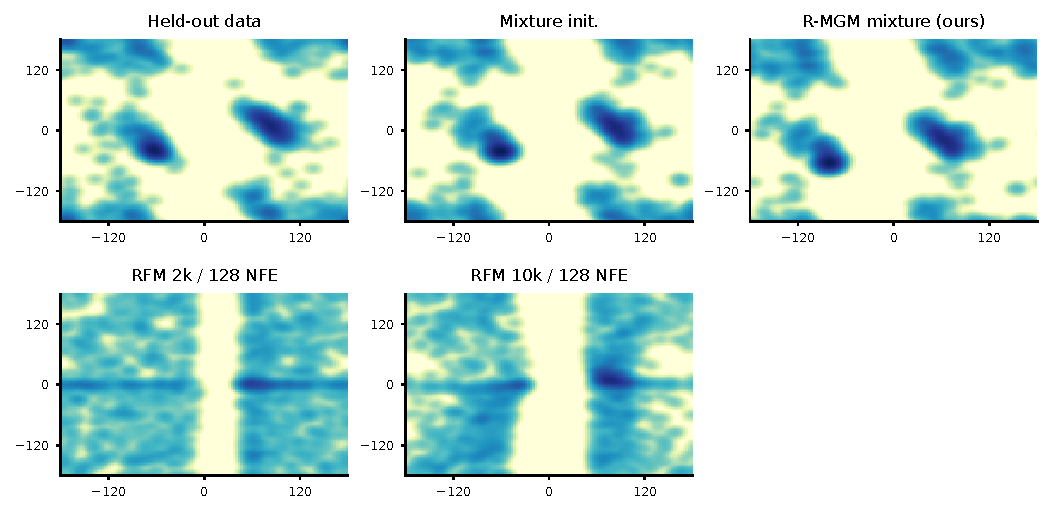
\includegraphics[width=\textwidth]{figures/glycine_comparison.pdf}
\caption{Glycine: fixed test target and training seed 0. Columns are labeled with their generator or flow training budget. Common-bandwidth sample KDEs use the same scale within this figure; these are not likelihood plots.}\label{fig:extra-glycine}\end{figure*}
Figure~\ref{fig:extra-proline} shows the fixed-seed comparison for Proline.
\begin{figure*}[t]\centering
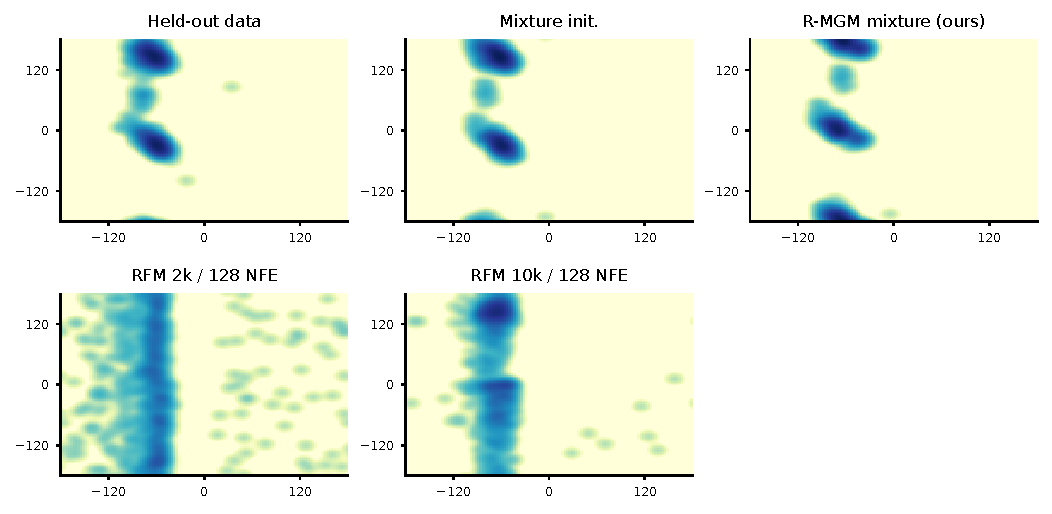
\includegraphics[width=\textwidth]{figures/proline_comparison.pdf}
\caption{Proline: fixed test target and training seed 0. Columns are labeled with their generator or flow training budget. Common-bandwidth sample KDEs use the same scale within this figure; these are not likelihood plots.}\label{fig:extra-proline}\end{figure*}
Figure~\ref{fig:extra-prepro} shows the fixed-seed comparison for Pre-Pro.
\begin{figure*}[t]\centering
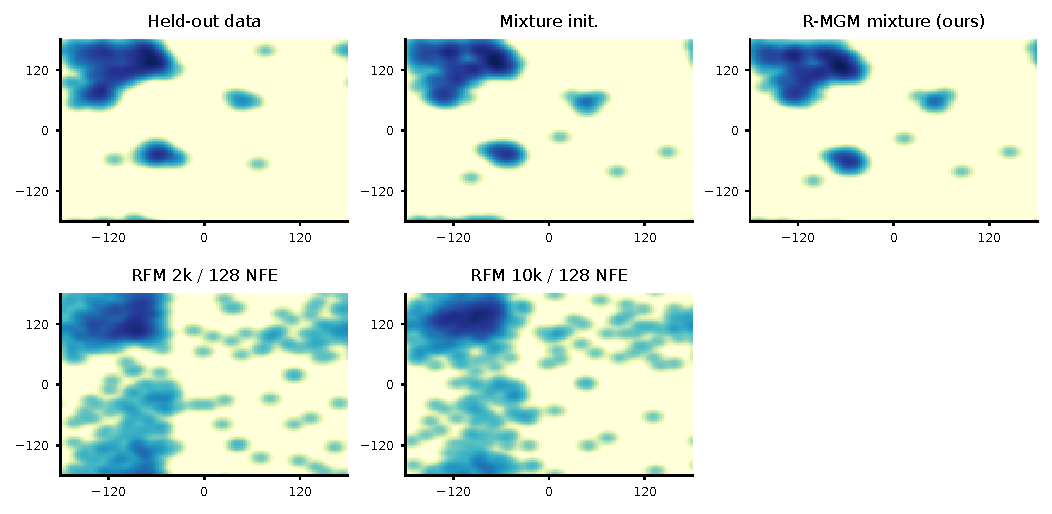
\includegraphics[width=\textwidth]{figures/prepro_comparison.pdf}
\caption{Pre-Pro: fixed test target and training seed 0. Columns are labeled with their generator or flow training budget. Common-bandwidth sample KDEs use the same scale within this figure; these are not likelihood plots.}\label{fig:extra-prepro}\end{figure*}
Figure~\ref{fig:extra-rna} shows the fixed-seed comparison for RNA (7D).
\begin{figure*}[t]\centering
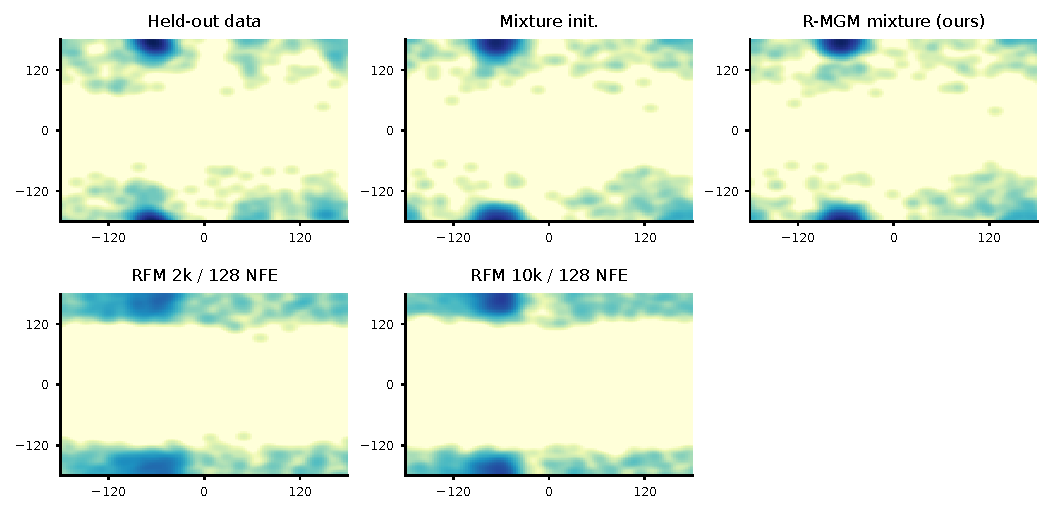
\includegraphics[width=\textwidth]{figures/rna_comparison.pdf}
\caption{RNA (7D): fixed test target and training seed 0. Columns are labeled with their generator or flow training budget. Common-bandwidth sample KDEs use the same scale within this figure; these are not likelihood plots.}\label{fig:extra-rna}\end{figure*}
\subsection{Final-Checkpoint Exploratory Mesh Results}
Each row is a single seed-0 model trained for 800 iterations. Values average three generated draws against the same 1,024 held-out targets. The plus/minus below is Monte Carlo sample SD, not training-seed variation. All kernels and coverage radii use a fixed training reference. The targets retain historical test exposure; final-checkpoint reevaluation does not erase it.
Table~\ref{tab:mesh} gives the final-checkpoint surface results.
\begin{table}[t]\caption{Exploratory mesh models: means and Monte Carlo SD over three draws from a single trained model per row. These are ambient sample metrics, not intrinsic likelihoods.}\label{tab:mesh}\centering\small\begin{tabular}{@{}llrrrr@{}}\toprule
Target & Generator & MMD$^2\times10^3$ & Ambient sym. NN & Coverage & Mean feasibility \\
\midrule
bunny10 & Projected mixture & $1.019\pm0.298$ & $0.043\pm0.000$ & $0.384\pm0.017$ & $2.8e-09$ \\
bunny10 & Soft sphere map & $33.905\pm0.992$ & $0.085\pm0.000$ & $0.248\pm0.012$ & $2.9e-09$ \\
bunny10 & Sphere-map mixture & $1.321\pm0.570$ & $0.042\pm0.000$ & $0.383\pm0.005$ & $3.1e-09$ \\
bunny100 & Projected mixture & $1.586\pm0.503$ & $0.063\pm0.001$ & $0.321\pm0.007$ & $3.2e-09$ \\
bunny100 & Soft sphere map & $75.212\pm7.842$ & $0.084\pm0.002$ & $0.161\pm0.007$ & $3.7e-09$ \\
bunny100 & Sphere-map mixture & $2.381\pm0.576$ & $0.056\pm0.001$ & $0.317\pm0.020$ & $3.1e-09$ \\
bunny50 & Projected mixture & $0.524\pm0.208$ & $0.043\pm0.001$ & $0.429\pm0.017$ & $2.7e-09$ \\
bunny50 & Soft sphere map & $53.416\pm2.984$ & $0.111\pm0.002$ & $0.158\pm0.014$ & $3.2e-09$ \\
bunny50 & Sphere-map mixture & $1.156\pm0.096$ & $0.048\pm0.001$ & $0.375\pm0.005$ & $2.9e-09$ \\
spot10 & Projected mixture & $0.751\pm0.398$ & $0.027\pm0.001$ & $0.453\pm0.035$ & $1.8e-09$ \\
spot10 & Soft sphere map & $47.778\pm1.717$ & $0.093\pm0.001$ & $0.189\pm0.004$ & $2.4e-09$ \\
spot10 & Sphere-map mixture & $1.167\pm0.601$ & $0.028\pm0.001$ & $0.444\pm0.013$ & $2.1e-09$ \\
spot100 & Projected mixture & $1.212\pm0.210$ & $0.052\pm0.002$ & $0.308\pm0.029$ & $2.8e-09$ \\
spot100 & Soft sphere map & $17.464\pm2.354$ & $0.061\pm0.002$ & $0.168\pm0.021$ & $2.8e-09$ \\
spot100 & Sphere-map mixture & $1.027\pm0.152$ & $0.047\pm0.001$ & $0.268\pm0.009$ & $2.8e-09$ \\
spot50 & Projected mixture & $1.897\pm0.666$ & $0.042\pm0.000$ & $0.388\pm0.008$ & $3.0e-09$ \\
spot50 & Soft sphere map & $35.720\pm3.309$ & $0.082\pm0.001$ & $0.153\pm0.010$ & $2.7e-09$ \\
spot50 & Sphere-map mixture & $2.516\pm0.586$ & $0.041\pm0.000$ & $0.385\pm0.005$ & $2.7e-09$ \\
\bottomrule\end{tabular}\end{table}
Surface feasibility measures mean distance to a second closest-point projection. It is not an intrinsic density metric or a certificate of bijective parameterization. The soft map interpolates radii from mesh-vertex directions and then projects; it is not the separate ray-intersection utility.
Figure~\ref{fig:surface-bunny10} gives the full parameterization comparison for bunny10.
\begin{figure*}[t]\centering
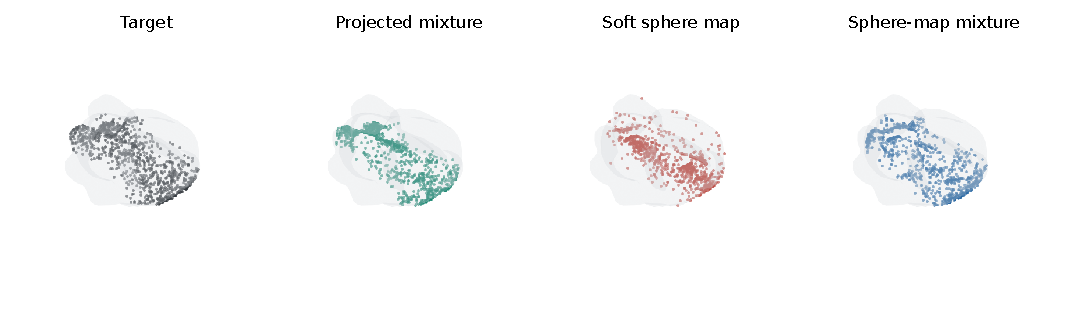
\includegraphics[width=\textwidth]{figures/bunny10_surface.pdf}
\caption{bunny10: one fixed seed-0 final checkpoint per variant, common cameras and 1,024 points. The loss is a local projection surrogate, not the spectral-path construction.}\label{fig:surface-bunny10}\end{figure*}
Figure~\ref{fig:surface-bunny50} gives the full parameterization comparison for bunny50.
\begin{figure*}[t]\centering
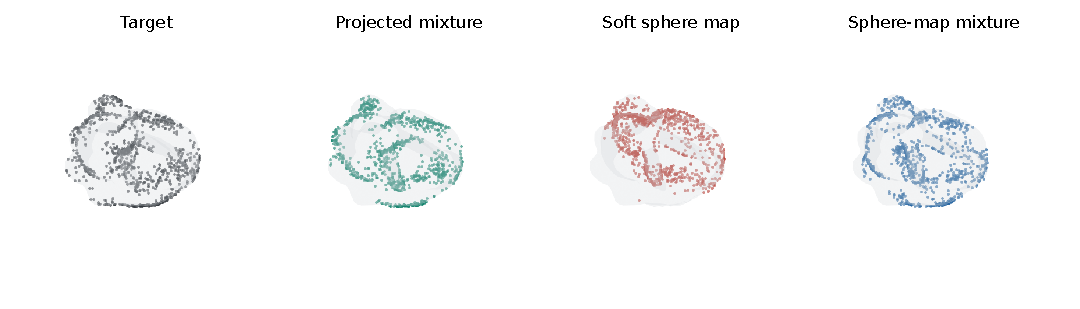
\includegraphics[width=\textwidth]{figures/bunny50_surface.pdf}
\caption{bunny50: one fixed seed-0 final checkpoint per variant, common cameras and 1,024 points. The loss is a local projection surrogate, not the spectral-path construction.}\label{fig:surface-bunny50}\end{figure*}
Figure~\ref{fig:surface-bunny100} gives the full parameterization comparison for bunny100.
\begin{figure*}[t]\centering
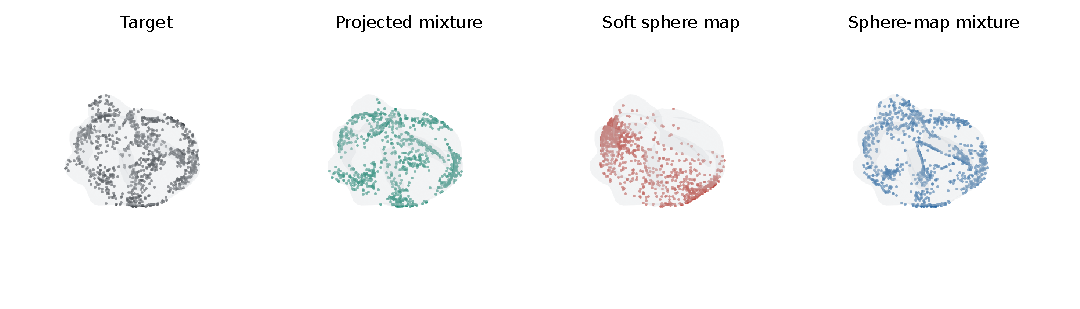
\includegraphics[width=\textwidth]{figures/bunny100_surface.pdf}
\caption{bunny100: one fixed seed-0 final checkpoint per variant, common cameras and 1,024 points. The loss is a local projection surrogate, not the spectral-path construction.}\label{fig:surface-bunny100}\end{figure*}
Figure~\ref{fig:surface-spot10} gives the full parameterization comparison for spot10.
\begin{figure*}[t]\centering
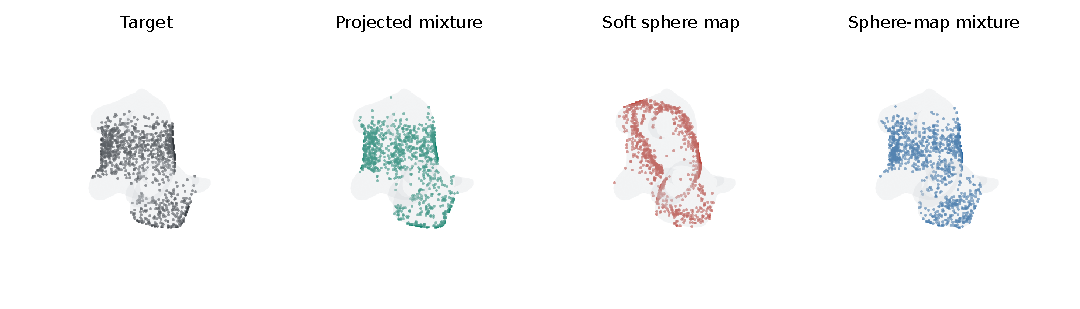
\includegraphics[width=\textwidth]{figures/spot10_surface.pdf}
\caption{spot10: one fixed seed-0 final checkpoint per variant, common cameras and 1,024 points. The loss is a local projection surrogate, not the spectral-path construction.}\label{fig:surface-spot10}\end{figure*}
Figure~\ref{fig:surface-spot50} gives the full parameterization comparison for spot50.
\begin{figure*}[t]\centering
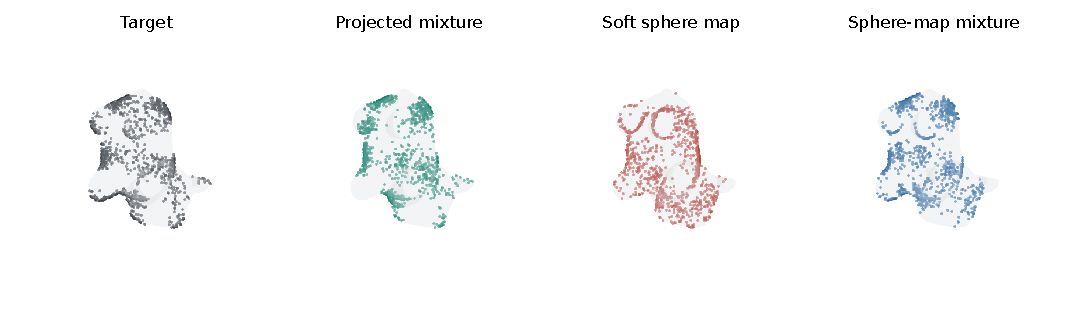
\includegraphics[width=\textwidth]{figures/spot50_surface.pdf}
\caption{spot50: one fixed seed-0 final checkpoint per variant, common cameras and 1,024 points. The loss is a local projection surrogate, not the spectral-path construction.}\label{fig:surface-spot50}\end{figure*}
Figure~\ref{fig:surface-spot100} gives the full parameterization comparison for spot100.
\begin{figure*}[t]\centering
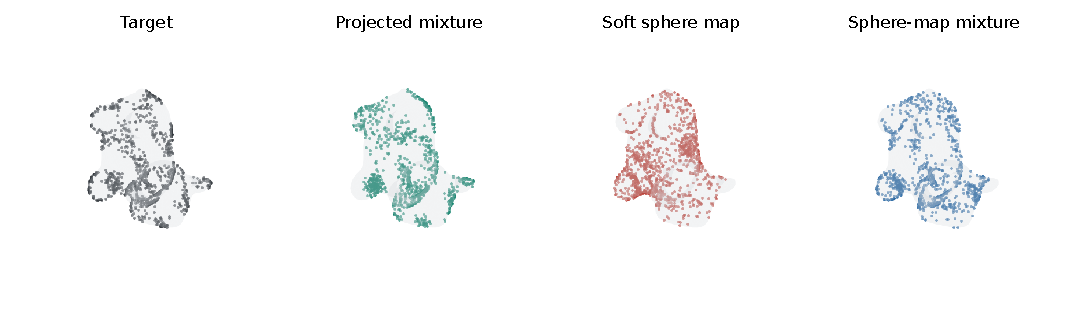
\includegraphics[width=\textwidth]{figures/spot100_surface.pdf}
\caption{spot100: one fixed seed-0 final checkpoint per variant, common cameras and 1,024 points. The loss is a local projection surrogate, not the spectral-path construction.}\label{fig:surface-spot100}\end{figure*}


\clearpage
\section{Scope Compared with the RFM Benchmark}
\label{app:inventory}
The evaluation includes the Earth event and protein/RNA angle tasks associated with the RFM code. They are distribution-learning tasks, not hazard prediction or molecular simulation. The closed-surface targets are positive-eigenfunction distributions on Bunny and Spot with target indices $10,50,100$. This target index differs from the number of spectral eigenfunctions used to construct an RFM path. A projection surrogate does not use spectral paths merely because its target data were generated from eigenfunctions.

Original real-data RFM configurations allow one million updates for Earth and protein/RNA. The existing original-code queue did not complete such runs; its presence is not evidence of completion. Controlled RFM rows use their own recorded architecture and budget. Small synthetic SPD cases are distinct from real EEG covariances: the $6\times6$, $25\times25$, and $59\times59$ EEG experiments are not reproduced here. Sample MMD is never substituted into a likelihood table.

Table~\ref{tab:benchmark-scope} records the distinction between shared data and a faithful reproduction of a published experiment.
\begin{table}[t]
\caption{Coverage of RFM experiment families. Using a reference target dataset does not imply matching its original model, geometry implementation, training budget, or likelihood evaluation.}
\label{tab:benchmark-scope}
\centering\small
\begin{tabular}{@{}p{.25\textwidth}p{.24\textwidth}p{.44\textwidth}@{}}
\toprule
Reference family & Present evidence & Important difference \\
\midrule
Earth data on $\mathbb S^2$ & Four controlled tasks, three seeds & Smaller RFM, 2k/10k updates; sample metrics, not author-budget NLL \\
Protein torsions on $\mathbb T^2$ & Four controlled tasks, three seeds & Row split; raw-angle primary fields; initialization and objective controls \\
RNA on $\mathbb T^7$ & Controlled task, three seeds & Local preprocessing count; same limited flow budget \\
Bunny and Spot surfaces & Six targets, three generator variants & One historical seed; projected-path surrogate; ambient sample metrics \\
Manifold with boundary / maze & Historical target-only pilot & Adapted source law and local projection; not the original transport task \\
High-dimensional scaling & Historical tori in dimensions 5, 10, 20 & Partial sweep, one seed, legacy estimator \\
Hyperbolic / additional geometries & Historical pilot and geometry checks & Target-only adaptation; approximate path velocity \\
Real EEG SPD covariances & Not completed & Synthetic small SPD pilots do not reproduce EEG results \\
\bottomrule
\end{tabular}
\end{table}

\section{Comparison of the Learning Constructions}
\label{app:comparisons}
Table~\ref{tab:constructions} contrasts the learned objects and training signals.
\begin{table}[t]
\caption{Relationship between geometric generative constructions. One-step inference alone is shared by several prior approaches.}
\label{tab:constructions}
\centering\small
\begin{tabular}{@{}p{.19\textwidth}p{.23\textwidth}p{.27\textwidth}p{.22\textwidth}@{}}
\toprule
Construction & Learned object & Defining training signal & Inference \\
\midrule
RFM \citep{chen2024general} & Time-dependent tangent field & Conditional geometric path-velocity regression & Integrate a learned field \\
Riemannian consistency / flow maps \citep{cheng2025rcm,davis2026gfm,woo2026rmf,zhong2026rmf} & Direct or two-time geometric map & Consistency, average-velocity, or flow-map identities & One or a few map evaluations \\
Intrinsic drifting / Wasserstein methods \citep{estebancasadevall2026kgdm,nurgulan2026rwflow,li2026rwgf} & Amortized generator & Kernel- or energy-induced distributional fields & One generator evaluation \\
R-MGM (ours) & Generator and tangent regression critic & Hidden-flip conditional moments at intermediate points & One generator evaluation \\
\bottomrule
\end{tabular}
\end{table}
This taxonomy specifies constructions rather than an empirical ranking. Some consistency methods admit both distillation and from-scratch training; one-step inference and the absence of a teacher alone do not distinguish our proposal. Population identifiability, energy dissipation, finite-horizon particle approximation, and convergence of finite neural training are different claims. They must be checked against the corresponding assumptions of each paper.

In particular, the midpoint critic is evaluated at a symmetrized intermediate location. Updating the generator requires derivatives through the path and its velocity, rather than simply applying the critic as a drift at the generated endpoint. A kernel-based particle update with a stop-gradient regression target implements a different optimization rule. A Wasserstein interpretation of any specific rule would require a first variation and a continuity-equation argument for its training-time dynamics. Our interpolation-current identity proves a distribution-discrepancy bound; it does not establish such an optimization-dynamics equivalence.

\section{Reproducibility and Computational Resources}
\label{app:reproduce}
The accompanying scripts generate tables from recorded machine-readable results and figures from sample arrays. The generated protocol lists commands, seeds, split identifiers, package versions, durations, and checkpoints. New GPU work uses one NVIDIA GeForce RTX 4090. Repeated Monte Carlo evaluations of one checkpoint are distinguished from independent training seeds. The PowerShell build script calls installed MiKTeX PDFLaTeX and BibTeX; unmodified ICML style files accompany the sources.

\paragraph{AI assistance.}
Generative AI tools assisted manuscript drafting, implementation, and internal error checking. They are not components of the evaluated generative models. The internal reviews are automated checks, not independent human peer review. Scientific validation and responsibility remain with the human authors.

\end{document}
